% Created 2025-01-28 ti 17:36
% Intended LaTeX compiler: pdflatex
\documentclass[12pt]{article}

%%%% settings when exporting code %%%% 

\usepackage{listings}
\lstdefinestyle{code-small}{
backgroundcolor=\color{white}, % background color for the code block
basicstyle=\ttfamily\small, % font used to display the code
commentstyle=\color[rgb]{0.5,0,0.5}, % color used to display comments in the code
keywordstyle=\color{black}, % color used to highlight certain words in the code
numberstyle=\ttfamily\tiny\color{gray}, % color used to display the line numbers
rulecolor=\color{black}, % color of the frame
stringstyle=\color[rgb]{0,.5,0},  % color used to display strings in the code
breakatwhitespace=false, % sets if automatic breaks should only happen at whitespace
breaklines=true, % sets automatic line breaking
columns=fullflexible,
frame=single, % adds a frame around the code (non,leftline,topline,bottomline,lines,single,shadowbox)
keepspaces=true, % % keeps spaces in text, useful for keeping indentation of code
literate={~}{$\sim$}{1}, % symbol properly display via latex
numbers=none, % where to put the line-numbers; possible values are (none, left, right)
numbersep=10pt, % how far the line-numbers are from the code
showspaces=false,
showstringspaces=false,
stepnumber=1, % the step between two line-numbers. If it's 1, each line will be numbered
tabsize=1,
xleftmargin=0cm,
emph={anova,apply,class,coef,colnames,colNames,colSums,dim,dcast,for,ggplot,head,if,ifelse,is.na,lapply,list.files,library,logLik,melt,plot,require,rowSums,sapply,setcolorder,setkey,str,summary,tapply},
aboveskip = \medskipamount, % define the space above displayed listings.
belowskip = \medskipamount, % define the space above displayed listings.
lineskip = 0pt} % specifies additional space between lines in listings
\lstset{style=code-small}
%%%% packages %%%%%

\usepackage[utf8]{inputenc}
\usepackage[T1]{fontenc}
\usepackage{lmodern}
\usepackage{textcomp}
\usepackage{color}
\usepackage{graphicx}
\usepackage{grffile}
\usepackage{wrapfig}
\usepackage{rotating}
\usepackage{longtable}
\usepackage{multirow}
\usepackage{multicol}
\usepackage{changes}
\usepackage{pdflscape}
\usepackage{geometry}
\usepackage[normalem]{ulem}
\usepackage{amssymb}
\usepackage{amsmath}
\usepackage{amsfonts}
\usepackage{dsfont}
\usepackage{array}
\usepackage{ifthen}
\usepackage{hyperref}
\usepackage{natbib}
\RequirePackage{setspace} % to modify the space between lines - incompatible with footnote in beamer
\renewcommand{\baselinestretch}{1.1}
\geometry{top=1cm}
\usepackage{titlesec}
\usepackage{etoolbox}

\makeatletter
\patchcmd{\ttlh@hang}{\parindent\z@}{\parindent\z@\leavevmode}{}{}
\patchcmd{\ttlh@hang}{\noindent}{}{}{}
\makeatother
\RequirePackage{colortbl} % arrayrulecolor to mix colors
\definecolor{myorange}{rgb}{1,0.2,0}
\definecolor{mypurple}{rgb}{0.7,0,8}
\definecolor{mycyan}{rgb}{0,0.6,0.6}
\newcommand{\lightblue}{blue!50!white}
\newcommand{\darkblue}{blue!80!black}
\newcommand{\darkgreen}{green!50!black}
\newcommand{\darkred}{red!50!black}
\definecolor{gray}{gray}{0.5}
\hypersetup{
citecolor=[rgb]{0,0.5,0},
urlcolor=[rgb]{0,0,0.5},
linkcolor=[rgb]{0,0,0.5},
}
\newenvironment{note}{\small \color{gray}\fontfamily{lmtt}\selectfont}{\par}
\newenvironment{activity}{\color{orange}\fontfamily{qzc}\selectfont}{\par}
\RequirePackage{pifont}
\RequirePackage{relsize}
\newcommand{\Cross}{{\raisebox{-0.5ex}%
{\relsize{1.5}\ding{56}}}\hspace{1pt} }
\newcommand{\Valid}{{\raisebox{-0.5ex}%
{\relsize{1.5}\ding{52}}}\hspace{1pt} }
\newcommand{\CrossR}{ \textcolor{red}{\Cross} }
\newcommand{\ValidV}{ \textcolor{green}{\Valid} }
\usepackage{stackengine}
\usepackage{scalerel}
\newcommand\Warning[1][3ex]{%
\renewcommand\stacktype{L}%
\scaleto{\stackon[1.3pt]{\color{red}$\triangle$}{\tiny\bfseries !}}{#1}%
\xspace
}
\definecolor{grayR}{HTML}{8A8990}
\definecolor{grayL}{HTML}{C4C7C9}
\definecolor{blueM}{HTML}{1F63B5}
\newcommand{\Rlogo}[1][0.07]{
\begin{tikzpicture}[scale=#1]
\shade [right color=grayR,left color=grayL,shading angle=60]
(-3.55,0.3) .. controls (-3.55,1.75)
and (-1.9,2.7) .. (0,2.7) .. controls (2.05,2.7)
and (3.5,1.6) .. (3.5,0.3) .. controls (3.5,-1.2)
and (1.55,-2) .. (0,-2) .. controls (-2.3,-2)
and (-3.55,-0.75) .. cycle;

\fill[white]
(-2.15,0.2) .. controls (-2.15,1.2)
and (-0.7,1.8) .. (0.5,1.8) .. controls (2.2,1.8)
and (3.1,1.2) .. (3.1,0.2) .. controls (3.1,-0.75)
and (2.4,-1.45) .. (0.5,-1.45) .. controls (-1.1,-1.45)
and (-2.15,-0.7) .. cycle;

\fill[blueM]
(1.75,1.25) -- (-0.65,1.25) -- (-0.65,-2.75) -- (0.55,-2.75) -- (0.55,-1.15) --
(0.95,-1.15)  .. controls (1.15,-1.15)
and (1.5,-1.9) .. (1.9,-2.75) -- (3.25,-2.75)  .. controls (2.2,-1)
and (2.5,-1.2) .. (1.8,-0.95) .. controls (2.6,-0.9)
and (2.85,-0.35) .. (2.85,0.2) .. controls (2.85,0.7)
and (2.5,1.2) .. cycle;

\fill[white]  (1.4,0.4) -- (0.55,0.4) -- (0.55,-0.3) -- (1.4,-0.3).. controls (1.75,-0.3)
and (1.75,0.4) .. cycle;

\end{tikzpicture}
}
\RequirePackage{fancyvrb}
\DefineVerbatimEnvironment{verbatim}{Verbatim}{fontsize=\small,formatcom = {\color[rgb]{0.5,0,0}}}
\RequirePackage{enumitem} % better than enumerate
\usepackage{float} %figure inside minipage
\RequirePackage{epstopdf} % to be able to convert .eps to .pdf image files
\RequirePackage{capt-of} %
\RequirePackage{caption} % newlines in graphics
\RequirePackage{tikz-cd} % graph
\RequirePackage{booktabs} % for nice lines in table (e.g. toprule, bottomrule, midrule, cmidrule)
\RequirePackage{amsmath}
\RequirePackage{algorithm}
\RequirePackage[noend]{algpseudocode}
\RequirePackage{dsfont}
\RequirePackage{amsmath,stmaryrd,graphicx}
\RequirePackage{prodint} % product integral symbol (\PRODI)
\usepackage{ifthen}
\usepackage{xifthen}
\usepackage{xargs}
\usepackage{xspace}
\newcommand\defOperator[7]{%
\ifthenelse{\isempty{#2}}{
\ifthenelse{\isempty{#1}}{#7{#3}#4}{#7{#3}#4 \left#5 #1 \right#6}
}{
\ifthenelse{\isempty{#1}}{#7{#3}#4_{#2}}{#7{#3}#4_{#1}\left#5 #2 \right#6}
}
}
\newcommand\defUOperator[5]{%
\ifthenelse{\isempty{#1}}{
#5\left#3 #2 \right#4
}{
\ifthenelse{\isempty{#2}}{\underset{#1}{\operatornamewithlimits{#5}}}{
\underset{#1}{\operatornamewithlimits{#5}}\left#3 #2 \right#4}
}
}
\newcommand{\defBoldVar}[2]{
\ifthenelse{\equal{#2}{T}}{\boldsymbol{#1}}{\mathbf{#1}}
}
\newcommandx\Esp[2][1=,2=]{\defOperator{#1}{#2}{E}{}{\lbrack}{\rbrack}{\mathbb}}
\newcommandx\Prob[2][1=,2=]{\defOperator{#1}{#2}{P}{}{\lbrack}{\rbrack}{\mathbb}}
\newcommandx\Qrob[2][1=,2=]{\defOperator{#1}{#2}{Q}{}{\lbrack}{\rbrack}{\mathbb}}
\newcommandx\Var[2][1=,2=]{\defOperator{#1}{#2}{V}{ar}{\lbrack}{\rbrack}{\mathbb}}
\newcommandx\Cov[2][1=,2=]{\defOperator{#1}{#2}{C}{ov}{\lbrack}{\rbrack}{\mathbb}}
\newcommandx\Binom[2][1=,2=]{\defOperator{#1}{#2}{B}{}{(}{)}{\mathcal}}
\newcommandx\Gaus[2][1=,2=]{\defOperator{#1}{#2}{N}{}{(}{)}{\mathcal}}
\newcommandx\Wishart[2][1=,2=]{\defOperator{#1}{#2}{W}{ishart}{(}{)}{\mathcal}}
\newcommandx\Likelihood[2][1=,2=]{\defOperator{#1}{#2}{L}{}{(}{)}{\mathcal}}
\newcommandx\logLikelihood[2][1=,2=]{\defOperator{#1}{#2}{\ell}{}{(}{)}{}}
\newcommandx\Information[2][1=,2=]{\defOperator{#1}{#2}{I}{}{(}{)}{\mathcal}}
\newcommandx\Score[2][1=,2=]{\defOperator{#1}{#2}{S}{}{(}{)}{\mathcal}}
\newcommandx\Vois[2][1=,2=]{\defOperator{#1}{#2}{V}{}{(}{)}{\mathcal}}
\newcommandx\IF[2][1=,2=]{\defOperator{#1}{#2}{IF}{}{(}{)}{\mathcal}}
\newcommandx\Ind[1][1=]{\defOperator{}{#1}{1}{}{(}{)}{\mathds}}
\newcommandx\Max[2][1=,2=]{\defUOperator{#1}{#2}{(}{)}{min}}
\newcommandx\Min[2][1=,2=]{\defUOperator{#1}{#2}{(}{)}{max}}
\newcommandx\argMax[2][1=,2=]{\defUOperator{#1}{#2}{(}{)}{argmax}}
\newcommandx\argMin[2][1=,2=]{\defUOperator{#1}{#2}{(}{)}{argmin}}
\newcommandx\cvD[2][1=D,2=n \rightarrow \infty]{\xrightarrow[#2]{#1}}
\newcommandx\Hypothesis[2][1=,2=]{
\ifthenelse{\isempty{#1}}{
\mathcal{H}
}{
\ifthenelse{\isempty{#2}}{
\mathcal{H}_{#1}
}{
\mathcal{H}^{(#2)}_{#1}
}
}
}
\newcommandx\dpartial[4][1=,2=,3=,4=\partial]{
\ifthenelse{\isempty{#3}}{
\frac{#4 #1}{#4 #2}
}{
\left.\frac{#4 #1}{#4 #2}\right\rvert_{#3}
}
}
\newcommandx\dTpartial[3][1=,2=,3=]{\dpartial[#1][#2][#3][d]}
\newcommandx\ddpartial[3][1=,2=,3=]{
\ifthenelse{\isempty{#3}}{
\frac{\partial^{2} #1}{\partial #2^2}
}{
\frac{\partial^2 #1}{\partial #2\partial #3}
}
}
\newcommand\Real{\mathbb{R}}
\newcommand\Rational{\mathbb{Q}}
\newcommand\Natural{\mathbb{N}}
\newcommand\trans[1]{{#1}^\intercal}%\newcommand\trans[1]{{\vphantom{#1}}^\top{#1}}
\newcommand{\independent}{\mathrel{\text{\scalebox{1.5}{$\perp\mkern-10mu\perp$}}}}
\newcommand\half{\frac{1}{2}}
\newcommand\normMax[1]{\left|\left|#1\right|\right|_{max}}
\newcommand\normTwo[1]{\left|\left|#1\right|\right|_{2}}
\newcommand\Veta{\boldsymbol{\eta}}
\newcommand\VX{\mathbf{X}}
\newcommand\sample{\chi}
\newcommand\Hspace{\mathcal{H}}
\newcommand\Tspace{\mathcal{T}}
\author{Brice Ozenne}
\date{\today}
\title{Handling deviation from normality}
\hypersetup{
 colorlinks=true,
 pdfauthor={Brice Ozenne},
 pdftitle={Handling deviation from normality},
 pdfkeywords={},
 pdfsubject={},
 pdfcreator={Emacs 27.2 (Org mode 9.5.2)},
 pdflang={English}
 }
\begin{document}

\maketitle
\noindent A question that often arise in consultations is:

\begin{center}
"My data is not normally distributed. What should I do?"
\end{center}

\noindent I find it difficult to answer as it is vague. It is a bit
like going to the doctor and asking him:

\begin{center}
 "My body temperature is outside of
the 36-37\textdegree C normal range. What should I do?"
\end{center}

\noindent In some cases statistical methods are robust (i.e. ensure
approximate type 1 error control and give nearly efficient estimators)
to "small" deviations from normality. So while it is a good idea to
check for normality, it is not a good idea to change statistical tool
just because you get a significant p-value out of a Shapiro test. If I
follow the analogy, medicine can be harmful and one should not take
medicine every time ones body temperature is outside the normal
range. It is however a good idea to check what is going on when your
temperature is high to make sure it does not hide something bad. First
thing to consider is the type of variable for which the concern about
normality arised:
\begin{itemize}
\item \textbf{outcome}: non-normality can be a threat to the interpretability
of the estimate and the validity of subsquent hypothesis
test. Example of non-normality are shown in \autoref{fig:examples}
and corresponding solution are discussed section \ref{sec:outcome}.
\item \textbf{exposure}: generally not a problem. One notable exception is in
presence of outliers when assuming a linear exposure effect as the
outliers may have an unacceptable influence on the exposure effect
(see \autoref{fig:leverage} for example). This will be discussed in
section \ref{sec:exposure}.
\item \textbf{covariate}: generally not a problem. One notable exception is in
presence of outliers when assuming a linear exposure effect as the
outliers may have an unacceptable influence on the exposure
effect. Possible solutions relaxing the linearity assumption
(using splines or categorizing the covariate). If the covariate is
not strongly related to the outcome one can also consider
excluding it from the model. It is not further discussed in this
document.
\end{itemize}

\noindent Before discussing any solution, the next section what is understood as
a 'good' or a 'valid' statistical procedure.

\clearpage

\section{Statistical properties}
\label{sec:properties}
When we use a statistical procedure to estimate a parameter of
interest (say \(\theta\)), we generally want to report an estimate of
this parameter based on the data we have (denoted
\(\widehat{\theta}\)). We generally also want to report the
uncertainty around this estimate via a confidence intervals (denoted
\(IC_{\widehat{\theta}} = [L_{\widehat{\theta}} ;
U_{\widehat{\theta}}]\)) or report a p-value that reflects whether a
value (say \(\theta_0\)) is compatible with the data at hand. We will
therefore distinguish three properties for a statistical procedure:
\begin{itemize}
\item \textbf{validity of the estimate}: the estimate should tend to the true
value as we increase the sample size (consistency) or the average
estimate should tend to the true value as repeat the
experiment (unbiasedness).
\item \textbf{validity of the uncertainty}: the confidence interval should have
proper coverage, typically they should contain the true value with
probablity 95\%. The p-value should have a uniform distribution under
the null meaning that the type 1 error is controlled at its nominal
level, typically 5\%.
\item \textbf{robustness}: means that the validity of the estimate and
uncertainty is not (dramatically) altered when the sample is altered
by a fixed proportion of extreme values (say 1\% of outliers).
\item \textbf{efficiency}: the procedure is optimal in the sense that it makes
the best use of the data at hand. \newline For instance we expect
the estimates to be as precise as possible, i.e. to have the
narrowest possible confidence intervals. We also expect that the
type 2 error should be the smallest possible (i.e. highest
power). In other terms, whenever the null hypothesis is false, the
test should rejected it as often as possible.
\end{itemize}

\bigskip

In the following we will assume that these properties are of
decreasing interest: having unbiased estimates is the most important
as quantifying uncertainty and efficiency can be fixed by
replicating studies and performing a meta-analysis. A non-efficient
estimator can still give useful and valid results - it will "just"
waste ressources but not be misleading (if used and interpreted
correctly). Typically robustness can be acquired at the expense of
efficiency (and interpretability).

\clearpage

\section{Non-normal exposure}
\label{sec:exposure}
Consider the following example shown in \autoref{fig:leverage} (example 5.1 in \cite{maronna2019robust}) evaluating the association between the
contents of Western Australian rocks. Consider first a \textbf{linear
relationship}:
\begin{itemize}
\item one point has a significant impact on the regression slope: 0.135
(p<0.001) vs 0.030 (p=0.18) when exluded. The 'red' regression line
does not seems to be a reasonnable summary of the association.
\item even after removal of observation 15, the exposure is still far from
following a normal distribution as it seems very
right-skewed. Nevertheless the 'blue' regression line seems to be a
reasonnable summary of the association.
\item modeling the median instead of the mean only partially solves the
issue: observation 15 has still a noticeable influence on the slope
(0.080 vs. 0.056). In fact in a more extreme example shown in the
right panel of As shown in \autoref{fig:leverageExtreme} one could
construct example where a small fraction of outliers would still be
very influencial.
\end{itemize}

\noindent Consider instead a \textbf{non-linear} relationship:
\begin{itemize}
\item using thin plate regression splines seems to provide a reasonnable
summary of the association with a different slope for small copper
value compared to high copper content. The later slope is probably
estimated with a lot of uncertainty due to only few observations
with high copper content: this could be seen from the width of the
confidence intervals of the regression line.
\end{itemize}

\vspace{-1cm}

\begin{minipage}{0.475\linewidth}
\begin{figure}[H]
\centering
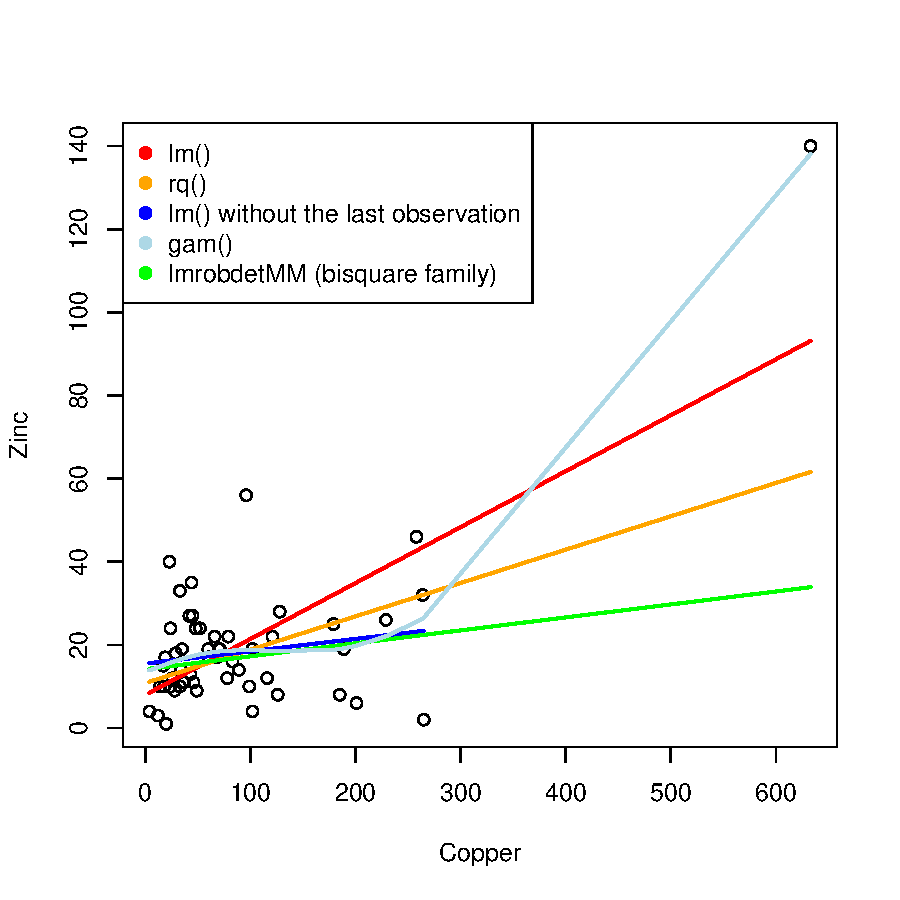
\includegraphics[width=\textwidth]{./figures/examples-leverage.pdf}
\caption{\label{fig:leverage}Real data with non-normal exposure.}
\end{figure}
\end{minipage}
\begin{minipage}{0.475\linewidth}
\begin{figure}[H]
\centering
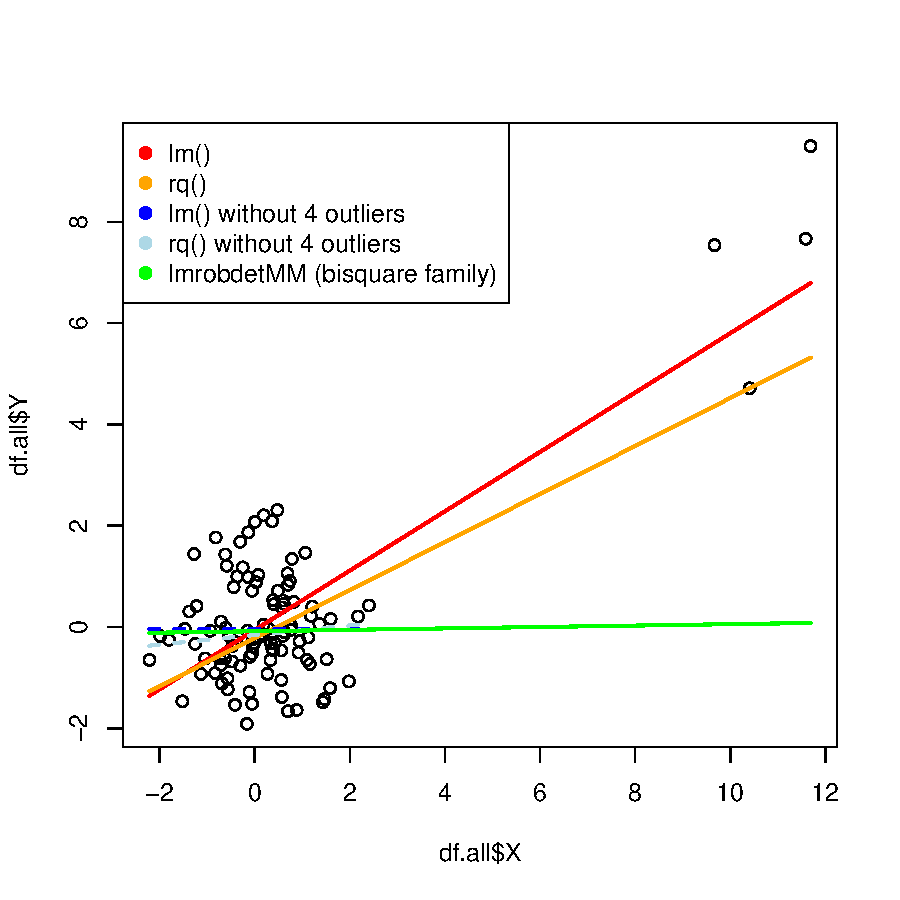
\includegraphics[width=\textwidth]{./figures/examplesExtreme-leverage.pdf}
\caption{\label{fig:leverageExtreme}Simulated data with non-normal exposure.}
\end{figure}

\end{minipage}

\clearpage

\noindent This example illustrate several key considerations:
\begin{itemize}
\item the exposure does not need to be normally distributed for
statistical methods to apply BUT parametric assumptions, such as
linearity, make common statistical tools sensitive to extreme
values.
\item it can be a good idea to restrict the study of the exposure to
commonly observed values. This is similar to an inclusion criteria in
a clinical trial on the disease severity (e.g. not including
terminally ill patients).
\item some methods sometimes refered as 'robust', like median or quantile
regression, have been developped to handle extreme values in the
outcome not in the exposure and thus may not lead to a satisfactory
solution. For instance, median regression minimizes the average of
the absolute residuals and can therefore be greatly influenced by a
single leverage point.
\item solutions include relaxing parametric assumptions or using more
specialized 'robust' technics, e.g. estimators based on a robust
summary of the residual (e.g. median of the absolute
residuals). They typically make the interpretation more challenging
either because there is no more a single number describing the
association or the single number is no more 'just' a mean or median
difference in the population of interest.
\end{itemize}


\subsection{\Rlogo code}
\label{sec:org2735878}

\subsubsection{No covariate}
\label{sec:orgf846aa9}

Load data:
\lstset{language=r,label= ,caption= ,captionpos=b,numbers=none}
\begin{lstlisting}
library(RobStatTM) 
data(mineral)
mineral <- mineral[order(mineral$copper),]
head(mineral)
\end{lstlisting}

\begin{verbatim}
   copper zinc
41      4    4
48     12    3
49     14   10
36     17   15
42     18   10
26     19   17
\end{verbatim}


Quick assessment of normality of the exposure:
\lstset{language=r,label= ,caption= ,captionpos=b,numbers=none}
\begin{lstlisting}
shapiro.test(mineral$copper)
\end{lstlisting}

\begin{verbatim}

	Shapiro-Wilk normality test

data:  mineral$copper
W = 0.67314, p-value = 1.374e-09
\end{verbatim}


Analysis:
\lstset{language=r,label= ,caption= ,captionpos=b,numbers=none}
\begin{lstlisting}
library(quantreg)
library(mgcv)
library(robust)
library(RobStatTM)

set.seed(1)
e.mean <- lm(zinc ~ copper, data = mineral)
e15.mean <- lm(zinc ~ copper, data = mineral[-NROW(mineral),])
e.median <- rq(zinc ~ copper, data = mineral)
e15.median <- rq(zinc ~ copper, data = mineral[-NROW(mineral),])
e.lmRob <- lmRob(zinc ~ copper, data = mineral)
e.lmRob2 <- lmrobdetMM(zinc ~ copper, data = mineral,
                       control = lmrobdet.control(family = "bisquare"))
e.gam <- gam(zinc ~ s(copper), data = mineral)

rbind(mean.all = summary(e.mean)$coef["copper",],
      median.all = summary(e.median, se = "boot")$coef["copper",],
      rob.all = summary(e.lmRob)$coef["copper",],
      rob2.all = summary(e.lmRob2)$coef["copper",],
      mean.red = summary(e15.mean)$coef["copper",],
      median.red = summary(e15.median, se = "boot")$coef["copper",])
\end{lstlisting}

\begin{verbatim}
             Estimate Std. Error   t value     Pr(>|t|)
mean.all   0.13456951 0.01982765 6.7869632 1.181421e-08
median.all 0.08024691 0.05326053 1.5066864 1.380606e-01
rob.all    0.01471517 0.02424047 0.6070496 5.465113e-01
rob2.all   0.03118872 0.02082673 1.4975332 1.404186e-01
mean.red   0.02974749 0.02205388 1.3488551 1.834611e-01
median.red 0.05590062 0.04380294 1.2761843 2.077867e-01
\end{verbatim}


\clearpage

\subsubsection{With covariates}
\label{sec:org511bc42}

We now consider a more complex example (example 5.2 in
\cite{maronna2019robust}) involving multiple covariates:
\lstset{language=r,label= ,caption= ,captionpos=b,numbers=none}
\begin{lstlisting}
library(robustbase) 
data(wood, package = "robustbase")
head(wood)
\end{lstlisting}

\begin{verbatim}
     x1     x2    x3    x4    x5     y
1 0.573 0.1059 0.465 0.538 0.841 0.534
2 0.651 0.1356 0.527 0.545 0.887 0.535
3 0.606 0.1273 0.494 0.521 0.920 0.570
4 0.437 0.1591 0.446 0.423 0.992 0.450
5 0.547 0.1135 0.531 0.519 0.915 0.548
6 0.444 0.1628 0.429 0.411 0.984 0.431
\end{verbatim}


\noindent We fit each model:
\lstset{language=r,label= ,caption= ,captionpos=b,numbers=none}
\begin{lstlisting}
e.lm <- lm(y ~ x1 + x2 + x3 + x4 + x5, data = wood)
e.lmRob2 <- lmrobdetMM(y ~ x1 + x2 + x3 + x4 + x5, data = wood,
                       control = lmrobdet.control(family = "bisquare"))
\end{lstlisting}

\noindent  And extract the partial residuals
\begin{itemize}
\item either adding the intercept and the contribution to the variable of
interest to the residuals:
\end{itemize}
\lstset{language=r,label= ,caption= ,captionpos=b,numbers=none}
\begin{lstlisting}
pres.lm <-  residuals(e.lm) + coef(e.lm)["(Intercept)"] + wood$x1 * coef(e.lm)["x1"]
pres.robust <- residuals(e.lmRob2) + coef(e.lmRob2)["(Intercept)"] + wood$x1 * coef(e.lmRob2)["x1"]
\end{lstlisting}

\begin{itemize}
\item or using the \texttt{residuals} method  and re-centering the result (to
match the original mean instead of 0):
\end{itemize}
\lstset{language=r,label= ,caption= ,captionpos=b,numbers=none}
\begin{lstlisting}
Mpres.lm2 <- residuals(e.lm, type = "partial")
centerX.lm <- sum(coef(e.lm)[paste0("x",2:5)] * colMeans(wood)[paste0("x",2:5)])
pres.lm2 <- Mpres.lm2[,"x1"] + attr(Mpres.lm2, "constant") - centerX.lm
\end{lstlisting}

Both approaches give the same up to a constant:
\lstset{language=r,label= ,caption= ,captionpos=b,numbers=none}
\begin{lstlisting}
range(pres.lm - pres.lm2)
\end{lstlisting}

\begin{verbatim}
[1] -1.110223e-16  1.110223e-16
\end{verbatim}


\noindent  We can then combine the partial residuals in a single data.frame:
\lstset{language=r,label= ,caption= ,captionpos=b,numbers=none}
\begin{lstlisting}
df.pres <- rbind(data.frame(method = "lm", x1 = wood2$x1, res = Mpres.lm),
                 data.frame(method = "robust", x1 = wood2$x1,
                            res = Mpres.robust))
\end{lstlisting}
and evaluate the model fit along x1 value, keep the other covariates at their reference level (here 0):
\lstset{language=r,label= ,caption= ,captionpos=b,numbers=none}
\begin{lstlisting}
grid.data <- data.frame(x1 = seq(min(wood2$x1),max(wood2$x1),by=0.01),
                        x2 = 0, x3 = 0, x4 = 0, x5 = 0)
df.pfit <- rbind(data.frame(method = "lm", x1 = grid.data$x1,
                            fit = predict(e.lm, newdata = grid.data)),
                 data.frame(method = "robust", x1 = grid.data$x1,
                            fit = predict(e.lmRob2, newdata = grid.data))
                 )
\end{lstlisting}

to obtain the following graphical display:
\lstset{language=r,label= ,caption= ,captionpos=b,numbers=none}
\begin{lstlisting}
library(ggplot2)
ggP <- ggplot(mapping = aes(x=x1))
ggP <- ggP + geom_point(data = df.pres,
                        mapping = aes(y = res, color = method))
ggP <- ggP + geom_line(data = df.pfit,
                       mapping = aes(y = fit, color = method))
ggP <- ggP + labs(x = "x1", y = "Y (partial residuals w.r.t. x1)")
ggP
\end{lstlisting}

\begin{center}
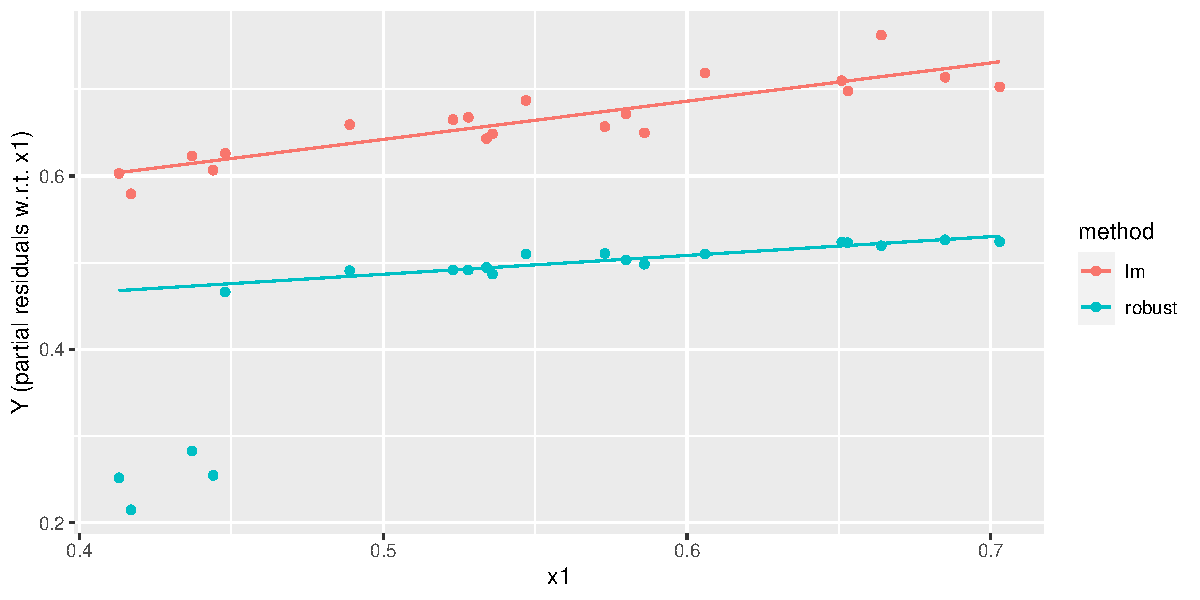
\includegraphics[trim={0 0 0 0},width=1\textwidth]{./figures/examples-covariates.pdf}
\label{fig:example-covariate}
\end{center}


\vspace{-1cm}

This dataset was created to have 4 unusual observations (those with
 \(x_1<0.45\)). The ordinary linear regression has the better overall
 fit (smaller variability of the residuals) whereas the robust
 approach has a better fit on the subset of 'usual' observations
 (smaller variability of the residuals when excluding the 4 unusual
 observations).

\clearpage

\section{Non-normal outcome}
\label{sec:outcome}
To ease the discussion, we will consider a simple example where we
want to compare the outcome distribution between two groups. We assume
to have no missing data and no measurement error, and that no external
covariate is relevant. In that case, we can visualize the distribution
of the outcome per group and perform the comparison "visually". We
will consider four examples (\autoref{fig:examples}):
\begin{itemize}
\item Normally distributed outcomes: no problem here.
\item Student distributed outcomes: symetric and unimodal distribution but with outliers.
\item Gamma distributed outcomes: asymetric distribution. A more extreme
distribution would show 'outliers'
\item Normally distributed outcomes with ceilling effect: many
observations have exactly the same value.
\end{itemize}

\Warning if any, distributional assumptions are usually made on the
residual terms, e.g:
\begin{align*}
Y = X \beta + \varepsilon \text{ where } \varepsilon \sim \Gaus[0,\sigma^2]
\end{align*}


and not on the outcome \(Y\). Concretely, we don't assume that the
outcome is normally distributed but that within groups (or once we
remove the group effect) it is normally distributed. In example 1, the
outcome is clearly not normally distributed (it is bimodal) but within
groups it is normally distributed.


\begin{figure}[H]
\centering
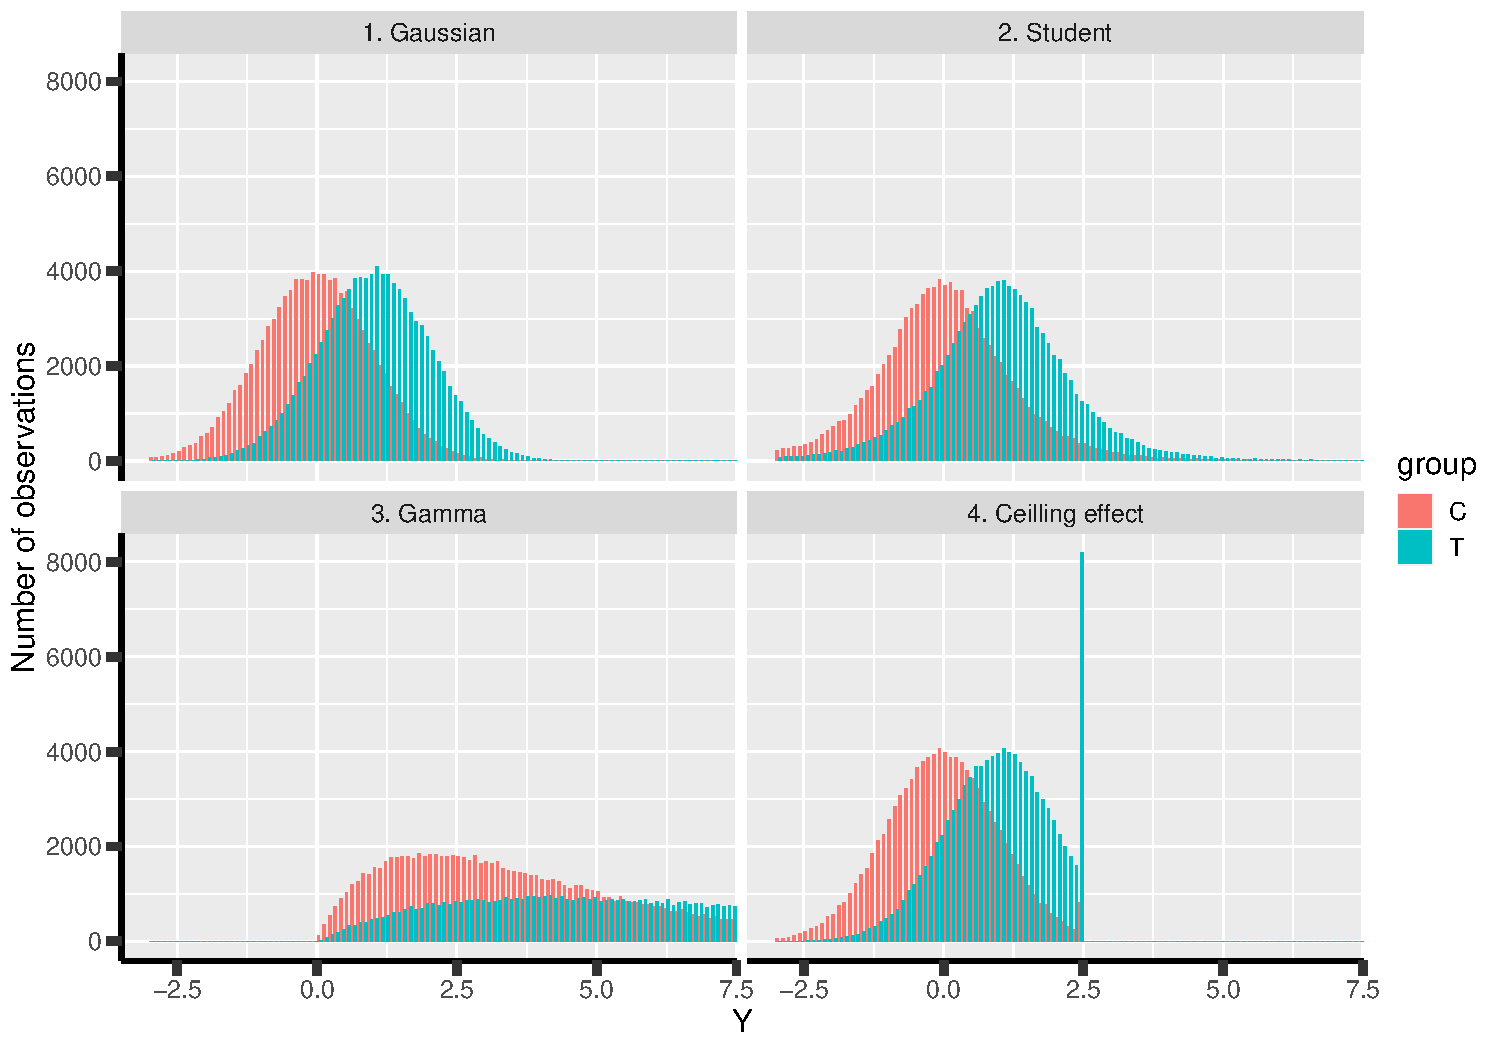
\includegraphics[width=\textwidth]{./figures/examples-hist.pdf}
\caption{\label{fig:examples}Example of simulated non-normal outcome.}
\end{figure}

\subsection{Should we worry about normality?}
\label{sec:org0f792e1}

Most statistical procedures do not require any normality assumption to
provide consistent estimates with asymptotically valid confidence
intervals and p-values. For instance t-tests and linear regressions
can be shown to provide consistent and asymptotically normally
distributed estimates in large iid \footnote{independent and identically
distributed} samples, regardless to whether they are normally
distributed as soon as their first two moments are finite\footnote{For some
statistical tests, this requires to use robust instead of model-based
standard error}. Here it is important to distringuish between the
distribution of the outcome (say \(Y\)) and the distribution of the
parameter of interest, often the mean of \(Y\). Averaging "normalizes"
the distribution, which is formalized in the central limit theorem,
and illustrated on \autoref{fig:distAverage}:

\begin{figure}[!h]
\centering
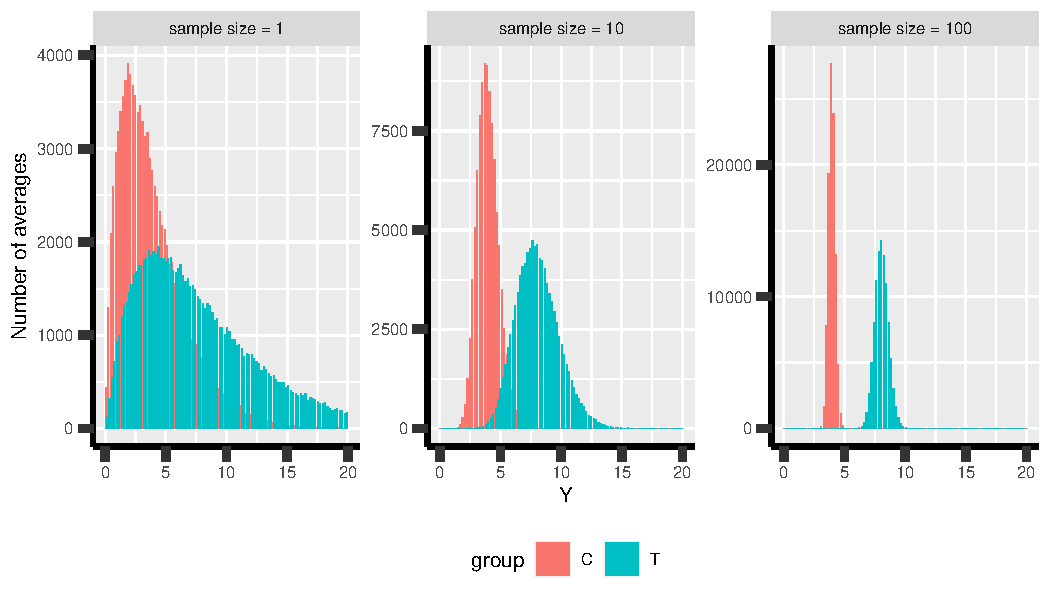
\includegraphics[width=\textwidth]{./figures/examples-histAverage.pdf}
\caption{\label{fig:distAverage}Distribution of the estimated mean along the sample size.}
\end{figure}

This means that (almost) regardless to the input data, we will be able
to estimate parameters which follows a normal distribution, i.e. for
which we can quantify the uncertainty. Results from the M-estimation
theory or the maximum likelihood theory can be used to show that
finding parameters that minimize an error that is the lack of fit
relative to individual observations lead to consistent
estimates. Concretely, this means that the coverage/type 1 error
control of many standard procedures such as the t-test and the linear
regression will be at their nominal level in large samples, even
though the normality assumption is not fullfilled
(\autoref{fig:coverage}) \ldots for large enough sample sizes.

\clearpage

\noindent Does that mean we should not worry about normality? No:
\begin{enumerate}
\item we may have a valid test / consistent estimate of a meaningless
parameter.
\item we may only have a small sample.
\item our estimator may not be efficient. This is usually not a problem,
except when we loose so much efficiency that the estimate becomes
very variable. This typically happen in presence of outliers.
\end{enumerate}
In the following we will discuss issues 1 to 3.

\begin{center}
\begin{tabular}{ll}
 & 0 \% \textasciitilde{}calculating\\
+ & 1 \% \textasciitilde{}11s\\
+ & 2 \% \textasciitilde{}11s\\
++ & 3 \% \textasciitilde{}11s\\
++ & 4 \% \textasciitilde{}10s\\
\sout{+} & 5 \% \textasciitilde{}10s\\
\sout{+} & 6 \% \textasciitilde{}10s\\
\sout{++} & 7 \% \textasciitilde{}10s\\
\sout{++} & 8 \% \textasciitilde{}10s\\
\sout{\sout{+}} & 9 \% \textasciitilde{}10s\\
\sout{\sout{+}} & 10\% \textasciitilde{}10s\\
\sout{\sout{++}} & 11\% \textasciitilde{}10s\\
\sout{\sout{++}} & 12\% \textasciitilde{}10s\\
\sout{\sout{\sout{+}}} & 13\% \textasciitilde{}10s\\
\sout{\sout{\sout{+}}} & 14\% \textasciitilde{}10s\\
\sout{\sout{\sout{++}}} & 15\% \textasciitilde{}09s\\
\sout{\sout{\sout{++}}} & 16\% \textasciitilde{}09s\\
\sout{\sout{\sout{\sout{+}}}} & 17\% \textasciitilde{}09s\\
\sout{\sout{\sout{\sout{+}}}} & 18\% \textasciitilde{}09s\\
\sout{\sout{\sout{\sout{++}}}} & 19\% \textasciitilde{}09s\\
\sout{\sout{\sout{\sout{++}}}} & 20\% \textasciitilde{}09s\\
\sout{\sout{\sout{\sout{\sout{+}}}}} & 21\% \textasciitilde{}09s\\
\sout{\sout{\sout{\sout{\sout{+}}}}} & 22\% \textasciitilde{}09s\\
\sout{\sout{\sout{\sout{\sout{++}}}}} & 23\% \textasciitilde{}09s\\
\sout{\sout{\sout{\sout{\sout{++}}}}} & 24\% \textasciitilde{}09s\\
\sout{\sout{\sout{\sout{\sout{\sout{+}}}}}} & 25\% \textasciitilde{}08s\\
\sout{\sout{\sout{\sout{\sout{\sout{+}}}}}} & 26\% \textasciitilde{}08s\\
\sout{\sout{\sout{\sout{\sout{\sout{++}}}}}} & 27\% \textasciitilde{}08s\\
\sout{\sout{\sout{\sout{\sout{\sout{++}}}}}} & 28\% \textasciitilde{}08s\\
\sout{\sout{\sout{\sout{\sout{\sout{\sout{+}}}}}}} & 29\% \textasciitilde{}08s\\
\sout{\sout{\sout{\sout{\sout{\sout{\sout{+}}}}}}} & 30\% \textasciitilde{}08s\\
\sout{\sout{\sout{\sout{\sout{\sout{\sout{++}}}}}}} & 31\% \textasciitilde{}08s\\
\sout{\sout{\sout{\sout{\sout{\sout{\sout{++}}}}}}} & 32\% \textasciitilde{}08s\\
\sout{\sout{\sout{\sout{\sout{\sout{\sout{\sout{+}}}}}}}} & 33\% \textasciitilde{}08s\\
\sout{\sout{\sout{\sout{\sout{\sout{\sout{\sout{+}}}}}}}} & 34\% \textasciitilde{}08s\\
\sout{\sout{\sout{\sout{\sout{\sout{\sout{\sout{++}}}}}}}} & 35\% \textasciitilde{}07s\\
\sout{\sout{\sout{\sout{\sout{\sout{\sout{\sout{++}}}}}}}} & 36\% \textasciitilde{}07s\\
\sout{\sout{\sout{\sout{\sout{\sout{\sout{\sout{\sout{+}}}}}}}}} & 37\% \textasciitilde{}07s\\
\sout{\sout{\sout{\sout{\sout{\sout{\sout{\sout{\sout{+}}}}}}}}} & 38\% \textasciitilde{}07s\\
\sout{\sout{\sout{\sout{\sout{\sout{\sout{\sout{\sout{++}}}}}}}}} & 39\% \textasciitilde{}07s\\
\sout{\sout{\sout{\sout{\sout{\sout{\sout{\sout{\sout{++}}}}}}}}} & 40\% \textasciitilde{}07s\\
\sout{\sout{\sout{\sout{\sout{\sout{\sout{\sout{\sout{\sout{+}}}}}}}}}} & 41\% \textasciitilde{}07s\\
\sout{\sout{\sout{\sout{\sout{\sout{\sout{\sout{\sout{\sout{+}}}}}}}}}} & 42\% \textasciitilde{}07s\\
\sout{\sout{\sout{\sout{\sout{\sout{\sout{\sout{\sout{\sout{++}}}}}}}}}} & 43\% \textasciitilde{}06s\\
\sout{\sout{\sout{\sout{\sout{\sout{\sout{\sout{\sout{\sout{++}}}}}}}}}} & 44\% \textasciitilde{}06s\\
\sout{\sout{\sout{\sout{\sout{\sout{\sout{\sout{\sout{\sout{\sout{+}}}}}}}}}}} & 45\% \textasciitilde{}06s\\
\sout{\sout{\sout{\sout{\sout{\sout{\sout{\sout{\sout{\sout{\sout{+}}}}}}}}}}} & 46\% \textasciitilde{}06s\\
\sout{\sout{\sout{\sout{\sout{\sout{\sout{\sout{\sout{\sout{\sout{++}}}}}}}}}}} & 47\% \textasciitilde{}06s\\
\sout{\sout{\sout{\sout{\sout{\sout{\sout{\sout{\sout{\sout{\sout{++}}}}}}}}}}} & 48\% \textasciitilde{}06s\\
\sout{\sout{\sout{\sout{\sout{\sout{\sout{\sout{\sout{\sout{\sout{\sout{+}}}}}}}}}}}} & 49\% \textasciitilde{}06s\\
\sout{\sout{\sout{\sout{\sout{\sout{\sout{\sout{\sout{\sout{\sout{\sout{+}}}}}}}}}}}} & 50\% \textasciitilde{}06s\\
\sout{\sout{\sout{\sout{\sout{\sout{\sout{\sout{\sout{\sout{\sout{\sout{++}}}}}}}}}}}} & 51\% \textasciitilde{}06s\\
\sout{\sout{\sout{\sout{\sout{\sout{\sout{\sout{\sout{\sout{\sout{\sout{++}}}}}}}}}}}} & 52\% \textasciitilde{}06s\\
\sout{\sout{\sout{\sout{\sout{\sout{\sout{\sout{\sout{\sout{\sout{\sout{\sout{+}}}}}}}}}}}}} & 53\% \textasciitilde{}05s\\
\sout{\sout{\sout{\sout{\sout{\sout{\sout{\sout{\sout{\sout{\sout{\sout{\sout{+}}}}}}}}}}}}} & 54\% \textasciitilde{}05s\\
\sout{\sout{\sout{\sout{\sout{\sout{\sout{\sout{\sout{\sout{\sout{\sout{\sout{++}}}}}}}}}}}}} & 55\% \textasciitilde{}05s\\
\sout{\sout{\sout{\sout{\sout{\sout{\sout{\sout{\sout{\sout{\sout{\sout{\sout{++}}}}}}}}}}}}} & 56\% \textasciitilde{}05s\\
\sout{\sout{\sout{\sout{\sout{\sout{\sout{\sout{\sout{\sout{\sout{\sout{\sout{\sout{+}}}}}}}}}}}}}} & 57\% \textasciitilde{}05s\\
\sout{\sout{\sout{\sout{\sout{\sout{\sout{\sout{\sout{\sout{\sout{\sout{\sout{\sout{+}}}}}}}}}}}}}} & 58\% \textasciitilde{}05s\\
\sout{\sout{\sout{\sout{\sout{\sout{\sout{\sout{\sout{\sout{\sout{\sout{\sout{\sout{++}}}}}}}}}}}}}} & 59\% \textasciitilde{}05s\\
\sout{\sout{\sout{\sout{\sout{\sout{\sout{\sout{\sout{\sout{\sout{\sout{\sout{\sout{++}}}}}}}}}}}}}} & 60\% \textasciitilde{}05s\\
\sout{\sout{\sout{\sout{\sout{\sout{\sout{\sout{\sout{\sout{\sout{\sout{\sout{\sout{\sout{+}}}}}}}}}}}}}}} & 61\% \textasciitilde{}05s\\
\sout{\sout{\sout{\sout{\sout{\sout{\sout{\sout{\sout{\sout{\sout{\sout{\sout{\sout{\sout{+}}}}}}}}}}}}}}} & 62\% \textasciitilde{}04s\\
\sout{\sout{\sout{\sout{\sout{\sout{\sout{\sout{\sout{\sout{\sout{\sout{\sout{\sout{\sout{++}}}}}}}}}}}}}}} & 63\% \textasciitilde{}04s\\
\sout{\sout{\sout{\sout{\sout{\sout{\sout{\sout{\sout{\sout{\sout{\sout{\sout{\sout{\sout{++}}}}}}}}}}}}}}} & 64\% \textasciitilde{}04s\\
\sout{\sout{\sout{\sout{\sout{\sout{\sout{\sout{\sout{\sout{\sout{\sout{\sout{\sout{\sout{\sout{+}}}}}}}}}}}}}}}} & 65\% \textasciitilde{}04s\\
\sout{\sout{\sout{\sout{\sout{\sout{\sout{\sout{\sout{\sout{\sout{\sout{\sout{\sout{\sout{\sout{+}}}}}}}}}}}}}}}} & 66\% \textasciitilde{}04s\\
\sout{\sout{\sout{\sout{\sout{\sout{\sout{\sout{\sout{\sout{\sout{\sout{\sout{\sout{\sout{\sout{++}}}}}}}}}}}}}}}} & 67\% \textasciitilde{}04s\\
\sout{\sout{\sout{\sout{\sout{\sout{\sout{\sout{\sout{\sout{\sout{\sout{\sout{\sout{\sout{\sout{++}}}}}}}}}}}}}}}} & 68\% \textasciitilde{}04s\\
\sout{\sout{\sout{\sout{\sout{\sout{\sout{\sout{\sout{\sout{\sout{\sout{\sout{\sout{\sout{\sout{\sout{+}}}}}}}}}}}}}}}}} & 69\% \textasciitilde{}04s\\
\sout{\sout{\sout{\sout{\sout{\sout{\sout{\sout{\sout{\sout{\sout{\sout{\sout{\sout{\sout{\sout{\sout{+}}}}}}}}}}}}}}}}} & 70\% \textasciitilde{}04s\\
\sout{\sout{\sout{\sout{\sout{\sout{\sout{\sout{\sout{\sout{\sout{\sout{\sout{\sout{\sout{\sout{\sout{++}}}}}}}}}}}}}}}}} & 71\% \textasciitilde{}04s\\
\sout{\sout{\sout{\sout{\sout{\sout{\sout{\sout{\sout{\sout{\sout{\sout{\sout{\sout{\sout{\sout{\sout{++}}}}}}}}}}}}}}}}} & 72\% \textasciitilde{}03s\\
\sout{\sout{\sout{\sout{\sout{\sout{\sout{\sout{\sout{\sout{\sout{\sout{\sout{\sout{\sout{\sout{\sout{\sout{+}}}}}}}}}}}}}}}}}} & 73\% \textasciitilde{}03s\\
\sout{\sout{\sout{\sout{\sout{\sout{\sout{\sout{\sout{\sout{\sout{\sout{\sout{\sout{\sout{\sout{\sout{\sout{+}}}}}}}}}}}}}}}}}} & 74\% \textasciitilde{}03s\\
\sout{\sout{\sout{\sout{\sout{\sout{\sout{\sout{\sout{\sout{\sout{\sout{\sout{\sout{\sout{\sout{\sout{\sout{++}}}}}}}}}}}}}}}}}} & 75\% \textasciitilde{}03s\\
\sout{\sout{\sout{\sout{\sout{\sout{\sout{\sout{\sout{\sout{\sout{\sout{\sout{\sout{\sout{\sout{\sout{\sout{++}}}}}}}}}}}}}}}}}} & 76\% \textasciitilde{}03s\\
\sout{\sout{\sout{\sout{\sout{\sout{\sout{\sout{\sout{\sout{\sout{\sout{\sout{\sout{\sout{\sout{\sout{\sout{\sout{+}}}}}}}}}}}}}}}}}}} & 77\% \textasciitilde{}03s\\
\sout{\sout{\sout{\sout{\sout{\sout{\sout{\sout{\sout{\sout{\sout{\sout{\sout{\sout{\sout{\sout{\sout{\sout{\sout{+}}}}}}}}}}}}}}}}}}} & 78\% \textasciitilde{}03s\\
\sout{\sout{\sout{\sout{\sout{\sout{\sout{\sout{\sout{\sout{\sout{\sout{\sout{\sout{\sout{\sout{\sout{\sout{\sout{++}}}}}}}}}}}}}}}}}}} & 79\% \textasciitilde{}03s\\
\sout{\sout{\sout{\sout{\sout{\sout{\sout{\sout{\sout{\sout{\sout{\sout{\sout{\sout{\sout{\sout{\sout{\sout{\sout{++}}}}}}}}}}}}}}}}}}} & 80\% \textasciitilde{}02s\\
\sout{\sout{\sout{\sout{\sout{\sout{\sout{\sout{\sout{\sout{\sout{\sout{\sout{\sout{\sout{\sout{\sout{\sout{\sout{\sout{+}}}}}}}}}}}}}}}}}}}} & 81\% \textasciitilde{}02s\\
\sout{\sout{\sout{\sout{\sout{\sout{\sout{\sout{\sout{\sout{\sout{\sout{\sout{\sout{\sout{\sout{\sout{\sout{\sout{\sout{+}}}}}}}}}}}}}}}}}}}} & 82\% \textasciitilde{}02s\\
\sout{\sout{\sout{\sout{\sout{\sout{\sout{\sout{\sout{\sout{\sout{\sout{\sout{\sout{\sout{\sout{\sout{\sout{\sout{\sout{++}}}}}}}}}}}}}}}}}}}} & 83\% \textasciitilde{}02s\\
\sout{\sout{\sout{\sout{\sout{\sout{\sout{\sout{\sout{\sout{\sout{\sout{\sout{\sout{\sout{\sout{\sout{\sout{\sout{\sout{++}}}}}}}}}}}}}}}}}}}} & 84\% \textasciitilde{}02s\\
\sout{\sout{\sout{\sout{\sout{\sout{\sout{\sout{\sout{\sout{\sout{\sout{\sout{\sout{\sout{\sout{\sout{\sout{\sout{\sout{\sout{+}}}}}}}}}}}}}}}}}}}}} & 85\% \textasciitilde{}02s\\
\sout{\sout{\sout{\sout{\sout{\sout{\sout{\sout{\sout{\sout{\sout{\sout{\sout{\sout{\sout{\sout{\sout{\sout{\sout{\sout{\sout{+}}}}}}}}}}}}}}}}}}}}} & 86\% \textasciitilde{}02s\\
\sout{\sout{\sout{\sout{\sout{\sout{\sout{\sout{\sout{\sout{\sout{\sout{\sout{\sout{\sout{\sout{\sout{\sout{\sout{\sout{\sout{++}}}}}}}}}}}}}}}}}}}}} & 87\% \textasciitilde{}02s\\
\sout{\sout{\sout{\sout{\sout{\sout{\sout{\sout{\sout{\sout{\sout{\sout{\sout{\sout{\sout{\sout{\sout{\sout{\sout{\sout{\sout{++}}}}}}}}}}}}}}}}}}}}} & 88\% \textasciitilde{}02s\\
\sout{\sout{\sout{\sout{\sout{\sout{\sout{\sout{\sout{\sout{\sout{\sout{\sout{\sout{\sout{\sout{\sout{\sout{\sout{\sout{\sout{\sout{+}}}}}}}}}}}}}}}}}}}}}} & 89\% \textasciitilde{}01s\\
\sout{\sout{\sout{\sout{\sout{\sout{\sout{\sout{\sout{\sout{\sout{\sout{\sout{\sout{\sout{\sout{\sout{\sout{\sout{\sout{\sout{\sout{+}}}}}}}}}}}}}}}}}}}}}} & 90\% \textasciitilde{}01s\\
\sout{\sout{\sout{\sout{\sout{\sout{\sout{\sout{\sout{\sout{\sout{\sout{\sout{\sout{\sout{\sout{\sout{\sout{\sout{\sout{\sout{\sout{++}}}}}}}}}}}}}}}}}}}}}} & 91\% \textasciitilde{}01s\\
\sout{\sout{\sout{\sout{\sout{\sout{\sout{\sout{\sout{\sout{\sout{\sout{\sout{\sout{\sout{\sout{\sout{\sout{\sout{\sout{\sout{\sout{++}}}}}}}}}}}}}}}}}}}}}} & 92\% \textasciitilde{}01s\\
\sout{\sout{\sout{\sout{\sout{\sout{\sout{\sout{\sout{\sout{\sout{\sout{\sout{\sout{\sout{\sout{\sout{\sout{\sout{\sout{\sout{\sout{\sout{+}}}}}}}}}}}}}}}}}}}}}}} & 93\% \textasciitilde{}01s\\
\sout{\sout{\sout{\sout{\sout{\sout{\sout{\sout{\sout{\sout{\sout{\sout{\sout{\sout{\sout{\sout{\sout{\sout{\sout{\sout{\sout{\sout{\sout{+}}}}}}}}}}}}}}}}}}}}}}} & 94\% \textasciitilde{}01s\\
\sout{\sout{\sout{\sout{\sout{\sout{\sout{\sout{\sout{\sout{\sout{\sout{\sout{\sout{\sout{\sout{\sout{\sout{\sout{\sout{\sout{\sout{\sout{++}}}}}}}}}}}}}}}}}}}}}}} & 95\% \textasciitilde{}01s\\
\sout{\sout{\sout{\sout{\sout{\sout{\sout{\sout{\sout{\sout{\sout{\sout{\sout{\sout{\sout{\sout{\sout{\sout{\sout{\sout{\sout{\sout{\sout{++}}}}}}}}}}}}}}}}}}}}}}} & 96\% \textasciitilde{}01s\\
\sout{\sout{\sout{\sout{\sout{\sout{\sout{\sout{\sout{\sout{\sout{\sout{\sout{\sout{\sout{\sout{\sout{\sout{\sout{\sout{\sout{\sout{\sout{\sout{+}}}}}}}}}}}}}}}}}}}}}}}} & 97\% \textasciitilde{}00s\\
\sout{\sout{\sout{\sout{\sout{\sout{\sout{\sout{\sout{\sout{\sout{\sout{\sout{\sout{\sout{\sout{\sout{\sout{\sout{\sout{\sout{\sout{\sout{\sout{+}}}}}}}}}}}}}}}}}}}}}}}} & 98\% \textasciitilde{}00s\\
\sout{\sout{\sout{\sout{\sout{\sout{\sout{\sout{\sout{\sout{\sout{\sout{\sout{\sout{\sout{\sout{\sout{\sout{\sout{\sout{\sout{\sout{\sout{\sout{++}}}}}}}}}}}}}}}}}}}}}}}} & 99\% \textasciitilde{}00s\\
\sout{\sout{\sout{\sout{\sout{\sout{\sout{\sout{\sout{\sout{\sout{\sout{\sout{\sout{\sout{\sout{\sout{\sout{\sout{\sout{\sout{\sout{\sout{\sout{++}}}}}}}}}}}}}}}}}}}}}}}} & 100\% elapsed=13s\\
\end{tabular}
\end{center}
\begin{verbatim}

\end{verbatim}

\begin{center}
\begin{tabular}{ll}
 & 0 \% \textasciitilde{}calculating\\
+ & 1 \% \textasciitilde{}11s\\
+ & 2 \% \textasciitilde{}12s\\
++ & 3 \% \textasciitilde{}12s\\
++ & 4 \% \textasciitilde{}12s\\
\sout{+} & 5 \% \textasciitilde{}11s\\
\sout{+} & 6 \% \textasciitilde{}11s\\
\sout{++} & 7 \% \textasciitilde{}11s\\
\sout{++} & 8 \% \textasciitilde{}11s\\
\sout{\sout{+}} & 9 \% \textasciitilde{}11s\\
\sout{\sout{+}} & 10\% \textasciitilde{}11s\\
\sout{\sout{++}} & 11\% \textasciitilde{}10s\\
\sout{\sout{++}} & 12\% \textasciitilde{}10s\\
\sout{\sout{\sout{+}}} & 13\% \textasciitilde{}10s\\
\sout{\sout{\sout{+}}} & 14\% \textasciitilde{}10s\\
\sout{\sout{\sout{++}}} & 15\% \textasciitilde{}10s\\
\sout{\sout{\sout{++}}} & 16\% \textasciitilde{}10s\\
\sout{\sout{\sout{\sout{+}}}} & 17\% \textasciitilde{}10s\\
\sout{\sout{\sout{\sout{+}}}} & 18\% \textasciitilde{}09s\\
\sout{\sout{\sout{\sout{++}}}} & 19\% \textasciitilde{}09s\\
\sout{\sout{\sout{\sout{++}}}} & 20\% \textasciitilde{}09s\\
\sout{\sout{\sout{\sout{\sout{+}}}}} & 21\% \textasciitilde{}09s\\
\sout{\sout{\sout{\sout{\sout{+}}}}} & 22\% \textasciitilde{}09s\\
\sout{\sout{\sout{\sout{\sout{++}}}}} & 23\% \textasciitilde{}09s\\
\sout{\sout{\sout{\sout{\sout{++}}}}} & 24\% \textasciitilde{}09s\\
\sout{\sout{\sout{\sout{\sout{\sout{+}}}}}} & 25\% \textasciitilde{}09s\\
\sout{\sout{\sout{\sout{\sout{\sout{+}}}}}} & 26\% \textasciitilde{}08s\\
\sout{\sout{\sout{\sout{\sout{\sout{++}}}}}} & 27\% \textasciitilde{}08s\\
\sout{\sout{\sout{\sout{\sout{\sout{++}}}}}} & 28\% \textasciitilde{}08s\\
\sout{\sout{\sout{\sout{\sout{\sout{\sout{+}}}}}}} & 29\% \textasciitilde{}08s\\
\sout{\sout{\sout{\sout{\sout{\sout{\sout{+}}}}}}} & 30\% \textasciitilde{}08s\\
\sout{\sout{\sout{\sout{\sout{\sout{\sout{++}}}}}}} & 31\% \textasciitilde{}08s\\
\sout{\sout{\sout{\sout{\sout{\sout{\sout{++}}}}}}} & 32\% \textasciitilde{}08s\\
\sout{\sout{\sout{\sout{\sout{\sout{\sout{\sout{+}}}}}}}} & 33\% \textasciitilde{}08s\\
\sout{\sout{\sout{\sout{\sout{\sout{\sout{\sout{+}}}}}}}} & 34\% \textasciitilde{}08s\\
\sout{\sout{\sout{\sout{\sout{\sout{\sout{\sout{++}}}}}}}} & 35\% \textasciitilde{}08s\\
\sout{\sout{\sout{\sout{\sout{\sout{\sout{\sout{++}}}}}}}} & 36\% \textasciitilde{}08s\\
\sout{\sout{\sout{\sout{\sout{\sout{\sout{\sout{\sout{+}}}}}}}}} & 37\% \textasciitilde{}08s\\
\sout{\sout{\sout{\sout{\sout{\sout{\sout{\sout{\sout{+}}}}}}}}} & 38\% \textasciitilde{}07s\\
\sout{\sout{\sout{\sout{\sout{\sout{\sout{\sout{\sout{++}}}}}}}}} & 39\% \textasciitilde{}07s\\
\sout{\sout{\sout{\sout{\sout{\sout{\sout{\sout{\sout{++}}}}}}}}} & 40\% \textasciitilde{}07s\\
\sout{\sout{\sout{\sout{\sout{\sout{\sout{\sout{\sout{\sout{+}}}}}}}}}} & 41\% \textasciitilde{}07s\\
\sout{\sout{\sout{\sout{\sout{\sout{\sout{\sout{\sout{\sout{+}}}}}}}}}} & 42\% \textasciitilde{}07s\\
\sout{\sout{\sout{\sout{\sout{\sout{\sout{\sout{\sout{\sout{++}}}}}}}}}} & 43\% \textasciitilde{}07s\\
\sout{\sout{\sout{\sout{\sout{\sout{\sout{\sout{\sout{\sout{++}}}}}}}}}} & 44\% \textasciitilde{}07s\\
\sout{\sout{\sout{\sout{\sout{\sout{\sout{\sout{\sout{\sout{\sout{+}}}}}}}}}}} & 45\% \textasciitilde{}07s\\
\sout{\sout{\sout{\sout{\sout{\sout{\sout{\sout{\sout{\sout{\sout{+}}}}}}}}}}} & 46\% \textasciitilde{}07s\\
\sout{\sout{\sout{\sout{\sout{\sout{\sout{\sout{\sout{\sout{\sout{++}}}}}}}}}}} & 47\% \textasciitilde{}06s\\
\sout{\sout{\sout{\sout{\sout{\sout{\sout{\sout{\sout{\sout{\sout{++}}}}}}}}}}} & 48\% \textasciitilde{}06s\\
\sout{\sout{\sout{\sout{\sout{\sout{\sout{\sout{\sout{\sout{\sout{\sout{+}}}}}}}}}}}} & 49\% \textasciitilde{}06s\\
\sout{\sout{\sout{\sout{\sout{\sout{\sout{\sout{\sout{\sout{\sout{\sout{+}}}}}}}}}}}} & 50\% \textasciitilde{}06s\\
\sout{\sout{\sout{\sout{\sout{\sout{\sout{\sout{\sout{\sout{\sout{\sout{++}}}}}}}}}}}} & 51\% \textasciitilde{}06s\\
\sout{\sout{\sout{\sout{\sout{\sout{\sout{\sout{\sout{\sout{\sout{\sout{++}}}}}}}}}}}} & 52\% \textasciitilde{}06s\\
\sout{\sout{\sout{\sout{\sout{\sout{\sout{\sout{\sout{\sout{\sout{\sout{\sout{+}}}}}}}}}}}}} & 53\% \textasciitilde{}06s\\
\sout{\sout{\sout{\sout{\sout{\sout{\sout{\sout{\sout{\sout{\sout{\sout{\sout{+}}}}}}}}}}}}} & 54\% \textasciitilde{}06s\\
\sout{\sout{\sout{\sout{\sout{\sout{\sout{\sout{\sout{\sout{\sout{\sout{\sout{++}}}}}}}}}}}}} & 55\% \textasciitilde{}06s\\
\sout{\sout{\sout{\sout{\sout{\sout{\sout{\sout{\sout{\sout{\sout{\sout{\sout{++}}}}}}}}}}}}} & 56\% \textasciitilde{}05s\\
\sout{\sout{\sout{\sout{\sout{\sout{\sout{\sout{\sout{\sout{\sout{\sout{\sout{\sout{+}}}}}}}}}}}}}} & 57\% \textasciitilde{}05s\\
\sout{\sout{\sout{\sout{\sout{\sout{\sout{\sout{\sout{\sout{\sout{\sout{\sout{\sout{+}}}}}}}}}}}}}} & 58\% \textasciitilde{}05s\\
\sout{\sout{\sout{\sout{\sout{\sout{\sout{\sout{\sout{\sout{\sout{\sout{\sout{\sout{++}}}}}}}}}}}}}} & 59\% \textasciitilde{}05s\\
\sout{\sout{\sout{\sout{\sout{\sout{\sout{\sout{\sout{\sout{\sout{\sout{\sout{\sout{++}}}}}}}}}}}}}} & 60\% \textasciitilde{}05s\\
\sout{\sout{\sout{\sout{\sout{\sout{\sout{\sout{\sout{\sout{\sout{\sout{\sout{\sout{\sout{+}}}}}}}}}}}}}}} & 61\% \textasciitilde{}05s\\
\sout{\sout{\sout{\sout{\sout{\sout{\sout{\sout{\sout{\sout{\sout{\sout{\sout{\sout{\sout{+}}}}}}}}}}}}}}} & 62\% \textasciitilde{}05s\\
\sout{\sout{\sout{\sout{\sout{\sout{\sout{\sout{\sout{\sout{\sout{\sout{\sout{\sout{\sout{++}}}}}}}}}}}}}}} & 63\% \textasciitilde{}05s\\
\sout{\sout{\sout{\sout{\sout{\sout{\sout{\sout{\sout{\sout{\sout{\sout{\sout{\sout{\sout{++}}}}}}}}}}}}}}} & 64\% \textasciitilde{}04s\\
\sout{\sout{\sout{\sout{\sout{\sout{\sout{\sout{\sout{\sout{\sout{\sout{\sout{\sout{\sout{\sout{+}}}}}}}}}}}}}}}} & 65\% \textasciitilde{}04s\\
\sout{\sout{\sout{\sout{\sout{\sout{\sout{\sout{\sout{\sout{\sout{\sout{\sout{\sout{\sout{\sout{+}}}}}}}}}}}}}}}} & 66\% \textasciitilde{}04s\\
\sout{\sout{\sout{\sout{\sout{\sout{\sout{\sout{\sout{\sout{\sout{\sout{\sout{\sout{\sout{\sout{++}}}}}}}}}}}}}}}} & 67\% \textasciitilde{}04s\\
\sout{\sout{\sout{\sout{\sout{\sout{\sout{\sout{\sout{\sout{\sout{\sout{\sout{\sout{\sout{\sout{++}}}}}}}}}}}}}}}} & 68\% \textasciitilde{}04s\\
\sout{\sout{\sout{\sout{\sout{\sout{\sout{\sout{\sout{\sout{\sout{\sout{\sout{\sout{\sout{\sout{\sout{+}}}}}}}}}}}}}}}}} & 69\% \textasciitilde{}04s\\
\sout{\sout{\sout{\sout{\sout{\sout{\sout{\sout{\sout{\sout{\sout{\sout{\sout{\sout{\sout{\sout{\sout{+}}}}}}}}}}}}}}}}} & 70\% \textasciitilde{}04s\\
\sout{\sout{\sout{\sout{\sout{\sout{\sout{\sout{\sout{\sout{\sout{\sout{\sout{\sout{\sout{\sout{\sout{++}}}}}}}}}}}}}}}}} & 71\% \textasciitilde{}04s\\
\sout{\sout{\sout{\sout{\sout{\sout{\sout{\sout{\sout{\sout{\sout{\sout{\sout{\sout{\sout{\sout{\sout{++}}}}}}}}}}}}}}}}} & 72\% \textasciitilde{}04s\\
\sout{\sout{\sout{\sout{\sout{\sout{\sout{\sout{\sout{\sout{\sout{\sout{\sout{\sout{\sout{\sout{\sout{\sout{+}}}}}}}}}}}}}}}}}} & 73\% \textasciitilde{}03s\\
\sout{\sout{\sout{\sout{\sout{\sout{\sout{\sout{\sout{\sout{\sout{\sout{\sout{\sout{\sout{\sout{\sout{\sout{+}}}}}}}}}}}}}}}}}} & 74\% \textasciitilde{}03s\\
\sout{\sout{\sout{\sout{\sout{\sout{\sout{\sout{\sout{\sout{\sout{\sout{\sout{\sout{\sout{\sout{\sout{\sout{++}}}}}}}}}}}}}}}}}} & 75\% \textasciitilde{}03s\\
\sout{\sout{\sout{\sout{\sout{\sout{\sout{\sout{\sout{\sout{\sout{\sout{\sout{\sout{\sout{\sout{\sout{\sout{++}}}}}}}}}}}}}}}}}} & 76\% \textasciitilde{}03s\\
\sout{\sout{\sout{\sout{\sout{\sout{\sout{\sout{\sout{\sout{\sout{\sout{\sout{\sout{\sout{\sout{\sout{\sout{\sout{+}}}}}}}}}}}}}}}}}}} & 77\% \textasciitilde{}03s\\
\sout{\sout{\sout{\sout{\sout{\sout{\sout{\sout{\sout{\sout{\sout{\sout{\sout{\sout{\sout{\sout{\sout{\sout{\sout{+}}}}}}}}}}}}}}}}}}} & 78\% \textasciitilde{}03s\\
\sout{\sout{\sout{\sout{\sout{\sout{\sout{\sout{\sout{\sout{\sout{\sout{\sout{\sout{\sout{\sout{\sout{\sout{\sout{++}}}}}}}}}}}}}}}}}}} & 79\% \textasciitilde{}03s\\
\sout{\sout{\sout{\sout{\sout{\sout{\sout{\sout{\sout{\sout{\sout{\sout{\sout{\sout{\sout{\sout{\sout{\sout{\sout{++}}}}}}}}}}}}}}}}}}} & 80\% \textasciitilde{}03s\\
\sout{\sout{\sout{\sout{\sout{\sout{\sout{\sout{\sout{\sout{\sout{\sout{\sout{\sout{\sout{\sout{\sout{\sout{\sout{\sout{+}}}}}}}}}}}}}}}}}}}} & 81\% \textasciitilde{}02s\\
\sout{\sout{\sout{\sout{\sout{\sout{\sout{\sout{\sout{\sout{\sout{\sout{\sout{\sout{\sout{\sout{\sout{\sout{\sout{\sout{+}}}}}}}}}}}}}}}}}}}} & 82\% \textasciitilde{}02s\\
\sout{\sout{\sout{\sout{\sout{\sout{\sout{\sout{\sout{\sout{\sout{\sout{\sout{\sout{\sout{\sout{\sout{\sout{\sout{\sout{++}}}}}}}}}}}}}}}}}}}} & 83\% \textasciitilde{}02s\\
\sout{\sout{\sout{\sout{\sout{\sout{\sout{\sout{\sout{\sout{\sout{\sout{\sout{\sout{\sout{\sout{\sout{\sout{\sout{\sout{++}}}}}}}}}}}}}}}}}}}} & 84\% \textasciitilde{}02s\\
\sout{\sout{\sout{\sout{\sout{\sout{\sout{\sout{\sout{\sout{\sout{\sout{\sout{\sout{\sout{\sout{\sout{\sout{\sout{\sout{\sout{+}}}}}}}}}}}}}}}}}}}}} & 85\% \textasciitilde{}02s\\
\sout{\sout{\sout{\sout{\sout{\sout{\sout{\sout{\sout{\sout{\sout{\sout{\sout{\sout{\sout{\sout{\sout{\sout{\sout{\sout{\sout{+}}}}}}}}}}}}}}}}}}}}} & 86\% \textasciitilde{}02s\\
\sout{\sout{\sout{\sout{\sout{\sout{\sout{\sout{\sout{\sout{\sout{\sout{\sout{\sout{\sout{\sout{\sout{\sout{\sout{\sout{\sout{++}}}}}}}}}}}}}}}}}}}}} & 87\% \textasciitilde{}02s\\
\sout{\sout{\sout{\sout{\sout{\sout{\sout{\sout{\sout{\sout{\sout{\sout{\sout{\sout{\sout{\sout{\sout{\sout{\sout{\sout{\sout{++}}}}}}}}}}}}}}}}}}}}} & 88\% \textasciitilde{}02s\\
\sout{\sout{\sout{\sout{\sout{\sout{\sout{\sout{\sout{\sout{\sout{\sout{\sout{\sout{\sout{\sout{\sout{\sout{\sout{\sout{\sout{\sout{+}}}}}}}}}}}}}}}}}}}}}} & 89\% \textasciitilde{}01s\\
\sout{\sout{\sout{\sout{\sout{\sout{\sout{\sout{\sout{\sout{\sout{\sout{\sout{\sout{\sout{\sout{\sout{\sout{\sout{\sout{\sout{\sout{+}}}}}}}}}}}}}}}}}}}}}} & 90\% \textasciitilde{}01s\\
\sout{\sout{\sout{\sout{\sout{\sout{\sout{\sout{\sout{\sout{\sout{\sout{\sout{\sout{\sout{\sout{\sout{\sout{\sout{\sout{\sout{\sout{++}}}}}}}}}}}}}}}}}}}}}} & 91\% \textasciitilde{}01s\\
\sout{\sout{\sout{\sout{\sout{\sout{\sout{\sout{\sout{\sout{\sout{\sout{\sout{\sout{\sout{\sout{\sout{\sout{\sout{\sout{\sout{\sout{++}}}}}}}}}}}}}}}}}}}}}} & 92\% \textasciitilde{}01s\\
\sout{\sout{\sout{\sout{\sout{\sout{\sout{\sout{\sout{\sout{\sout{\sout{\sout{\sout{\sout{\sout{\sout{\sout{\sout{\sout{\sout{\sout{\sout{+}}}}}}}}}}}}}}}}}}}}}}} & 93\% \textasciitilde{}01s\\
\sout{\sout{\sout{\sout{\sout{\sout{\sout{\sout{\sout{\sout{\sout{\sout{\sout{\sout{\sout{\sout{\sout{\sout{\sout{\sout{\sout{\sout{\sout{+}}}}}}}}}}}}}}}}}}}}}}} & 94\% \textasciitilde{}01s\\
\sout{\sout{\sout{\sout{\sout{\sout{\sout{\sout{\sout{\sout{\sout{\sout{\sout{\sout{\sout{\sout{\sout{\sout{\sout{\sout{\sout{\sout{\sout{++}}}}}}}}}}}}}}}}}}}}}}} & 95\% \textasciitilde{}01s\\
\sout{\sout{\sout{\sout{\sout{\sout{\sout{\sout{\sout{\sout{\sout{\sout{\sout{\sout{\sout{\sout{\sout{\sout{\sout{\sout{\sout{\sout{\sout{++}}}}}}}}}}}}}}}}}}}}}}} & 96\% \textasciitilde{}01s\\
\sout{\sout{\sout{\sout{\sout{\sout{\sout{\sout{\sout{\sout{\sout{\sout{\sout{\sout{\sout{\sout{\sout{\sout{\sout{\sout{\sout{\sout{\sout{\sout{+}}}}}}}}}}}}}}}}}}}}}}}} & 97\% \textasciitilde{}00s\\
\sout{\sout{\sout{\sout{\sout{\sout{\sout{\sout{\sout{\sout{\sout{\sout{\sout{\sout{\sout{\sout{\sout{\sout{\sout{\sout{\sout{\sout{\sout{\sout{+}}}}}}}}}}}}}}}}}}}}}}}} & 98\% \textasciitilde{}00s\\
\sout{\sout{\sout{\sout{\sout{\sout{\sout{\sout{\sout{\sout{\sout{\sout{\sout{\sout{\sout{\sout{\sout{\sout{\sout{\sout{\sout{\sout{\sout{\sout{++}}}}}}}}}}}}}}}}}}}}}}}} & 99\% \textasciitilde{}00s\\
\sout{\sout{\sout{\sout{\sout{\sout{\sout{\sout{\sout{\sout{\sout{\sout{\sout{\sout{\sout{\sout{\sout{\sout{\sout{\sout{\sout{\sout{\sout{\sout{++}}}}}}}}}}}}}}}}}}}}}}}} & 100\% elapsed=14s\\
\end{tabular}
\end{center}
\begin{verbatim}

\end{verbatim}

\begin{center}
\begin{tabular}{ll}
 & 0 \% \textasciitilde{}calculating\\
+ & 1 \% \textasciitilde{}12s\\
+ & 2 \% \textasciitilde{}12s\\
++ & 3 \% \textasciitilde{}12s\\
++ & 4 \% \textasciitilde{}12s\\
\sout{+} & 5 \% \textasciitilde{}12s\\
\sout{+} & 6 \% \textasciitilde{}12s\\
\sout{++} & 7 \% \textasciitilde{}12s\\
\sout{++} & 8 \% \textasciitilde{}11s\\
\sout{\sout{+}} & 9 \% \textasciitilde{}11s\\
\sout{\sout{+}} & 10\% \textasciitilde{}11s\\
\sout{\sout{++}} & 11\% \textasciitilde{}11s\\
\sout{\sout{++}} & 12\% \textasciitilde{}11s\\
\sout{\sout{\sout{+}}} & 13\% \textasciitilde{}11s\\
\sout{\sout{\sout{+}}} & 14\% \textasciitilde{}11s\\
\sout{\sout{\sout{++}}} & 15\% \textasciitilde{}11s\\
\sout{\sout{\sout{++}}} & 16\% \textasciitilde{}10s\\
\sout{\sout{\sout{\sout{+}}}} & 17\% \textasciitilde{}10s\\
\sout{\sout{\sout{\sout{+}}}} & 18\% \textasciitilde{}10s\\
\sout{\sout{\sout{\sout{++}}}} & 19\% \textasciitilde{}10s\\
\sout{\sout{\sout{\sout{++}}}} & 20\% \textasciitilde{}10s\\
\sout{\sout{\sout{\sout{\sout{+}}}}} & 21\% \textasciitilde{}10s\\
\sout{\sout{\sout{\sout{\sout{+}}}}} & 22\% \textasciitilde{}10s\\
\sout{\sout{\sout{\sout{\sout{++}}}}} & 23\% \textasciitilde{}10s\\
\sout{\sout{\sout{\sout{\sout{++}}}}} & 24\% \textasciitilde{}10s\\
\sout{\sout{\sout{\sout{\sout{\sout{+}}}}}} & 25\% \textasciitilde{}09s\\
\sout{\sout{\sout{\sout{\sout{\sout{+}}}}}} & 26\% \textasciitilde{}09s\\
\sout{\sout{\sout{\sout{\sout{\sout{++}}}}}} & 27\% \textasciitilde{}09s\\
\sout{\sout{\sout{\sout{\sout{\sout{++}}}}}} & 28\% \textasciitilde{}09s\\
\sout{\sout{\sout{\sout{\sout{\sout{\sout{+}}}}}}} & 29\% \textasciitilde{}09s\\
\sout{\sout{\sout{\sout{\sout{\sout{\sout{+}}}}}}} & 30\% \textasciitilde{}09s\\
\sout{\sout{\sout{\sout{\sout{\sout{\sout{++}}}}}}} & 31\% \textasciitilde{}09s\\
\sout{\sout{\sout{\sout{\sout{\sout{\sout{++}}}}}}} & 32\% \textasciitilde{}08s\\
\sout{\sout{\sout{\sout{\sout{\sout{\sout{\sout{+}}}}}}}} & 33\% \textasciitilde{}08s\\
\sout{\sout{\sout{\sout{\sout{\sout{\sout{\sout{+}}}}}}}} & 34\% \textasciitilde{}08s\\
\sout{\sout{\sout{\sout{\sout{\sout{\sout{\sout{++}}}}}}}} & 35\% \textasciitilde{}08s\\
\sout{\sout{\sout{\sout{\sout{\sout{\sout{\sout{++}}}}}}}} & 36\% \textasciitilde{}08s\\
\sout{\sout{\sout{\sout{\sout{\sout{\sout{\sout{\sout{+}}}}}}}}} & 37\% \textasciitilde{}08s\\
\sout{\sout{\sout{\sout{\sout{\sout{\sout{\sout{\sout{+}}}}}}}}} & 38\% \textasciitilde{}08s\\
\sout{\sout{\sout{\sout{\sout{\sout{\sout{\sout{\sout{++}}}}}}}}} & 39\% \textasciitilde{}08s\\
\sout{\sout{\sout{\sout{\sout{\sout{\sout{\sout{\sout{++}}}}}}}}} & 40\% \textasciitilde{}08s\\
\sout{\sout{\sout{\sout{\sout{\sout{\sout{\sout{\sout{\sout{+}}}}}}}}}} & 41\% \textasciitilde{}07s\\
\sout{\sout{\sout{\sout{\sout{\sout{\sout{\sout{\sout{\sout{+}}}}}}}}}} & 42\% \textasciitilde{}07s\\
\sout{\sout{\sout{\sout{\sout{\sout{\sout{\sout{\sout{\sout{++}}}}}}}}}} & 43\% \textasciitilde{}07s\\
\sout{\sout{\sout{\sout{\sout{\sout{\sout{\sout{\sout{\sout{++}}}}}}}}}} & 44\% \textasciitilde{}07s\\
\sout{\sout{\sout{\sout{\sout{\sout{\sout{\sout{\sout{\sout{\sout{+}}}}}}}}}}} & 45\% \textasciitilde{}07s\\
\sout{\sout{\sout{\sout{\sout{\sout{\sout{\sout{\sout{\sout{\sout{+}}}}}}}}}}} & 46\% \textasciitilde{}07s\\
\sout{\sout{\sout{\sout{\sout{\sout{\sout{\sout{\sout{\sout{\sout{++}}}}}}}}}}} & 47\% \textasciitilde{}07s\\
\sout{\sout{\sout{\sout{\sout{\sout{\sout{\sout{\sout{\sout{\sout{++}}}}}}}}}}} & 48\% \textasciitilde{}07s\\
\sout{\sout{\sout{\sout{\sout{\sout{\sout{\sout{\sout{\sout{\sout{\sout{+}}}}}}}}}}}} & 49\% \textasciitilde{}06s\\
\sout{\sout{\sout{\sout{\sout{\sout{\sout{\sout{\sout{\sout{\sout{\sout{+}}}}}}}}}}}} & 50\% \textasciitilde{}06s\\
\sout{\sout{\sout{\sout{\sout{\sout{\sout{\sout{\sout{\sout{\sout{\sout{++}}}}}}}}}}}} & 51\% \textasciitilde{}06s\\
\sout{\sout{\sout{\sout{\sout{\sout{\sout{\sout{\sout{\sout{\sout{\sout{++}}}}}}}}}}}} & 52\% \textasciitilde{}06s\\
\sout{\sout{\sout{\sout{\sout{\sout{\sout{\sout{\sout{\sout{\sout{\sout{\sout{+}}}}}}}}}}}}} & 53\% \textasciitilde{}06s\\
\sout{\sout{\sout{\sout{\sout{\sout{\sout{\sout{\sout{\sout{\sout{\sout{\sout{+}}}}}}}}}}}}} & 54\% \textasciitilde{}06s\\
\sout{\sout{\sout{\sout{\sout{\sout{\sout{\sout{\sout{\sout{\sout{\sout{\sout{++}}}}}}}}}}}}} & 55\% \textasciitilde{}06s\\
\sout{\sout{\sout{\sout{\sout{\sout{\sout{\sout{\sout{\sout{\sout{\sout{\sout{++}}}}}}}}}}}}} & 56\% \textasciitilde{}06s\\
\sout{\sout{\sout{\sout{\sout{\sout{\sout{\sout{\sout{\sout{\sout{\sout{\sout{\sout{+}}}}}}}}}}}}}} & 57\% \textasciitilde{}05s\\
\sout{\sout{\sout{\sout{\sout{\sout{\sout{\sout{\sout{\sout{\sout{\sout{\sout{\sout{+}}}}}}}}}}}}}} & 58\% \textasciitilde{}05s\\
\sout{\sout{\sout{\sout{\sout{\sout{\sout{\sout{\sout{\sout{\sout{\sout{\sout{\sout{++}}}}}}}}}}}}}} & 59\% \textasciitilde{}05s\\
\sout{\sout{\sout{\sout{\sout{\sout{\sout{\sout{\sout{\sout{\sout{\sout{\sout{\sout{++}}}}}}}}}}}}}} & 60\% \textasciitilde{}05s\\
\sout{\sout{\sout{\sout{\sout{\sout{\sout{\sout{\sout{\sout{\sout{\sout{\sout{\sout{\sout{+}}}}}}}}}}}}}}} & 61\% \textasciitilde{}05s\\
\sout{\sout{\sout{\sout{\sout{\sout{\sout{\sout{\sout{\sout{\sout{\sout{\sout{\sout{\sout{+}}}}}}}}}}}}}}} & 62\% \textasciitilde{}05s\\
\sout{\sout{\sout{\sout{\sout{\sout{\sout{\sout{\sout{\sout{\sout{\sout{\sout{\sout{\sout{++}}}}}}}}}}}}}}} & 63\% \textasciitilde{}05s\\
\sout{\sout{\sout{\sout{\sout{\sout{\sout{\sout{\sout{\sout{\sout{\sout{\sout{\sout{\sout{++}}}}}}}}}}}}}}} & 64\% \textasciitilde{}05s\\
\sout{\sout{\sout{\sout{\sout{\sout{\sout{\sout{\sout{\sout{\sout{\sout{\sout{\sout{\sout{\sout{+}}}}}}}}}}}}}}}} & 65\% \textasciitilde{}04s\\
\sout{\sout{\sout{\sout{\sout{\sout{\sout{\sout{\sout{\sout{\sout{\sout{\sout{\sout{\sout{\sout{+}}}}}}}}}}}}}}}} & 66\% \textasciitilde{}04s\\
\sout{\sout{\sout{\sout{\sout{\sout{\sout{\sout{\sout{\sout{\sout{\sout{\sout{\sout{\sout{\sout{++}}}}}}}}}}}}}}}} & 67\% \textasciitilde{}04s\\
\sout{\sout{\sout{\sout{\sout{\sout{\sout{\sout{\sout{\sout{\sout{\sout{\sout{\sout{\sout{\sout{++}}}}}}}}}}}}}}}} & 68\% \textasciitilde{}04s\\
\sout{\sout{\sout{\sout{\sout{\sout{\sout{\sout{\sout{\sout{\sout{\sout{\sout{\sout{\sout{\sout{\sout{+}}}}}}}}}}}}}}}}} & 69\% \textasciitilde{}04s\\
\sout{\sout{\sout{\sout{\sout{\sout{\sout{\sout{\sout{\sout{\sout{\sout{\sout{\sout{\sout{\sout{\sout{+}}}}}}}}}}}}}}}}} & 70\% \textasciitilde{}04s\\
\sout{\sout{\sout{\sout{\sout{\sout{\sout{\sout{\sout{\sout{\sout{\sout{\sout{\sout{\sout{\sout{\sout{++}}}}}}}}}}}}}}}}} & 71\% \textasciitilde{}04s\\
\sout{\sout{\sout{\sout{\sout{\sout{\sout{\sout{\sout{\sout{\sout{\sout{\sout{\sout{\sout{\sout{\sout{++}}}}}}}}}}}}}}}}} & 72\% \textasciitilde{}04s\\
\sout{\sout{\sout{\sout{\sout{\sout{\sout{\sout{\sout{\sout{\sout{\sout{\sout{\sout{\sout{\sout{\sout{\sout{+}}}}}}}}}}}}}}}}}} & 73\% \textasciitilde{}03s\\
\sout{\sout{\sout{\sout{\sout{\sout{\sout{\sout{\sout{\sout{\sout{\sout{\sout{\sout{\sout{\sout{\sout{\sout{+}}}}}}}}}}}}}}}}}} & 74\% \textasciitilde{}03s\\
\sout{\sout{\sout{\sout{\sout{\sout{\sout{\sout{\sout{\sout{\sout{\sout{\sout{\sout{\sout{\sout{\sout{\sout{++}}}}}}}}}}}}}}}}}} & 75\% \textasciitilde{}03s\\
\sout{\sout{\sout{\sout{\sout{\sout{\sout{\sout{\sout{\sout{\sout{\sout{\sout{\sout{\sout{\sout{\sout{\sout{++}}}}}}}}}}}}}}}}}} & 76\% \textasciitilde{}03s\\
\sout{\sout{\sout{\sout{\sout{\sout{\sout{\sout{\sout{\sout{\sout{\sout{\sout{\sout{\sout{\sout{\sout{\sout{\sout{+}}}}}}}}}}}}}}}}}}} & 77\% \textasciitilde{}03s\\
\sout{\sout{\sout{\sout{\sout{\sout{\sout{\sout{\sout{\sout{\sout{\sout{\sout{\sout{\sout{\sout{\sout{\sout{\sout{+}}}}}}}}}}}}}}}}}}} & 78\% \textasciitilde{}03s\\
\sout{\sout{\sout{\sout{\sout{\sout{\sout{\sout{\sout{\sout{\sout{\sout{\sout{\sout{\sout{\sout{\sout{\sout{\sout{++}}}}}}}}}}}}}}}}}}} & 79\% \textasciitilde{}03s\\
\sout{\sout{\sout{\sout{\sout{\sout{\sout{\sout{\sout{\sout{\sout{\sout{\sout{\sout{\sout{\sout{\sout{\sout{\sout{++}}}}}}}}}}}}}}}}}}} & 80\% \textasciitilde{}03s\\
\sout{\sout{\sout{\sout{\sout{\sout{\sout{\sout{\sout{\sout{\sout{\sout{\sout{\sout{\sout{\sout{\sout{\sout{\sout{\sout{+}}}}}}}}}}}}}}}}}}}} & 81\% \textasciitilde{}02s\\
\sout{\sout{\sout{\sout{\sout{\sout{\sout{\sout{\sout{\sout{\sout{\sout{\sout{\sout{\sout{\sout{\sout{\sout{\sout{\sout{+}}}}}}}}}}}}}}}}}}}} & 82\% \textasciitilde{}02s\\
\sout{\sout{\sout{\sout{\sout{\sout{\sout{\sout{\sout{\sout{\sout{\sout{\sout{\sout{\sout{\sout{\sout{\sout{\sout{\sout{++}}}}}}}}}}}}}}}}}}}} & 83\% \textasciitilde{}02s\\
\sout{\sout{\sout{\sout{\sout{\sout{\sout{\sout{\sout{\sout{\sout{\sout{\sout{\sout{\sout{\sout{\sout{\sout{\sout{\sout{++}}}}}}}}}}}}}}}}}}}} & 84\% \textasciitilde{}02s\\
\sout{\sout{\sout{\sout{\sout{\sout{\sout{\sout{\sout{\sout{\sout{\sout{\sout{\sout{\sout{\sout{\sout{\sout{\sout{\sout{\sout{+}}}}}}}}}}}}}}}}}}}}} & 85\% \textasciitilde{}02s\\
\sout{\sout{\sout{\sout{\sout{\sout{\sout{\sout{\sout{\sout{\sout{\sout{\sout{\sout{\sout{\sout{\sout{\sout{\sout{\sout{\sout{+}}}}}}}}}}}}}}}}}}}}} & 86\% \textasciitilde{}02s\\
\sout{\sout{\sout{\sout{\sout{\sout{\sout{\sout{\sout{\sout{\sout{\sout{\sout{\sout{\sout{\sout{\sout{\sout{\sout{\sout{\sout{++}}}}}}}}}}}}}}}}}}}}} & 87\% \textasciitilde{}02s\\
\sout{\sout{\sout{\sout{\sout{\sout{\sout{\sout{\sout{\sout{\sout{\sout{\sout{\sout{\sout{\sout{\sout{\sout{\sout{\sout{\sout{++}}}}}}}}}}}}}}}}}}}}} & 88\% \textasciitilde{}02s\\
\sout{\sout{\sout{\sout{\sout{\sout{\sout{\sout{\sout{\sout{\sout{\sout{\sout{\sout{\sout{\sout{\sout{\sout{\sout{\sout{\sout{\sout{+}}}}}}}}}}}}}}}}}}}}}} & 89\% \textasciitilde{}01s\\
\sout{\sout{\sout{\sout{\sout{\sout{\sout{\sout{\sout{\sout{\sout{\sout{\sout{\sout{\sout{\sout{\sout{\sout{\sout{\sout{\sout{\sout{+}}}}}}}}}}}}}}}}}}}}}} & 90\% \textasciitilde{}01s\\
\sout{\sout{\sout{\sout{\sout{\sout{\sout{\sout{\sout{\sout{\sout{\sout{\sout{\sout{\sout{\sout{\sout{\sout{\sout{\sout{\sout{\sout{++}}}}}}}}}}}}}}}}}}}}}} & 91\% \textasciitilde{}01s\\
\sout{\sout{\sout{\sout{\sout{\sout{\sout{\sout{\sout{\sout{\sout{\sout{\sout{\sout{\sout{\sout{\sout{\sout{\sout{\sout{\sout{\sout{++}}}}}}}}}}}}}}}}}}}}}} & 92\% \textasciitilde{}01s\\
\sout{\sout{\sout{\sout{\sout{\sout{\sout{\sout{\sout{\sout{\sout{\sout{\sout{\sout{\sout{\sout{\sout{\sout{\sout{\sout{\sout{\sout{\sout{+}}}}}}}}}}}}}}}}}}}}}}} & 93\% \textasciitilde{}01s\\
\sout{\sout{\sout{\sout{\sout{\sout{\sout{\sout{\sout{\sout{\sout{\sout{\sout{\sout{\sout{\sout{\sout{\sout{\sout{\sout{\sout{\sout{\sout{+}}}}}}}}}}}}}}}}}}}}}}} & 94\% \textasciitilde{}01s\\
\sout{\sout{\sout{\sout{\sout{\sout{\sout{\sout{\sout{\sout{\sout{\sout{\sout{\sout{\sout{\sout{\sout{\sout{\sout{\sout{\sout{\sout{\sout{++}}}}}}}}}}}}}}}}}}}}}}} & 95\% \textasciitilde{}01s\\
\sout{\sout{\sout{\sout{\sout{\sout{\sout{\sout{\sout{\sout{\sout{\sout{\sout{\sout{\sout{\sout{\sout{\sout{\sout{\sout{\sout{\sout{\sout{++}}}}}}}}}}}}}}}}}}}}}}} & 96\% \textasciitilde{}01s\\
\sout{\sout{\sout{\sout{\sout{\sout{\sout{\sout{\sout{\sout{\sout{\sout{\sout{\sout{\sout{\sout{\sout{\sout{\sout{\sout{\sout{\sout{\sout{\sout{+}}}}}}}}}}}}}}}}}}}}}}}} & 97\% \textasciitilde{}00s\\
\sout{\sout{\sout{\sout{\sout{\sout{\sout{\sout{\sout{\sout{\sout{\sout{\sout{\sout{\sout{\sout{\sout{\sout{\sout{\sout{\sout{\sout{\sout{\sout{+}}}}}}}}}}}}}}}}}}}}}}}} & 98\% \textasciitilde{}00s\\
\sout{\sout{\sout{\sout{\sout{\sout{\sout{\sout{\sout{\sout{\sout{\sout{\sout{\sout{\sout{\sout{\sout{\sout{\sout{\sout{\sout{\sout{\sout{\sout{++}}}}}}}}}}}}}}}}}}}}}}}} & 99\% \textasciitilde{}00s\\
\sout{\sout{\sout{\sout{\sout{\sout{\sout{\sout{\sout{\sout{\sout{\sout{\sout{\sout{\sout{\sout{\sout{\sout{\sout{\sout{\sout{\sout{\sout{\sout{++}}}}}}}}}}}}}}}}}}}}}}}} & 100\% elapsed=14s\\
\end{tabular}
\end{center}
\begin{verbatim}

\end{verbatim}

\begin{center}
\begin{tabular}{ll}
 & 0 \% \textasciitilde{}calculating\\
+ & 1 \% \textasciitilde{}12s\\
+ & 2 \% \textasciitilde{}13s\\
++ & 3 \% \textasciitilde{}12s\\
++ & 4 \% \textasciitilde{}13s\\
\sout{+} & 5 \% \textasciitilde{}13s\\
\sout{+} & 6 \% \textasciitilde{}12s\\
\sout{++} & 7 \% \textasciitilde{}12s\\
\sout{++} & 8 \% \textasciitilde{}12s\\
\sout{\sout{+}} & 9 \% \textasciitilde{}12s\\
\sout{\sout{+}} & 10\% \textasciitilde{}11s\\
\sout{\sout{++}} & 11\% \textasciitilde{}11s\\
\sout{\sout{++}} & 12\% \textasciitilde{}11s\\
\sout{\sout{\sout{+}}} & 13\% \textasciitilde{}11s\\
\sout{\sout{\sout{+}}} & 14\% \textasciitilde{}11s\\
\sout{\sout{\sout{++}}} & 15\% \textasciitilde{}11s\\
\sout{\sout{\sout{++}}} & 16\% \textasciitilde{}11s\\
\sout{\sout{\sout{\sout{+}}}} & 17\% \textasciitilde{}11s\\
\sout{\sout{\sout{\sout{+}}}} & 18\% \textasciitilde{}10s\\
\sout{\sout{\sout{\sout{++}}}} & 19\% \textasciitilde{}10s\\
\sout{\sout{\sout{\sout{++}}}} & 20\% \textasciitilde{}10s\\
\sout{\sout{\sout{\sout{\sout{+}}}}} & 21\% \textasciitilde{}10s\\
\sout{\sout{\sout{\sout{\sout{+}}}}} & 22\% \textasciitilde{}10s\\
\sout{\sout{\sout{\sout{\sout{++}}}}} & 23\% \textasciitilde{}10s\\
\sout{\sout{\sout{\sout{\sout{++}}}}} & 24\% \textasciitilde{}10s\\
\sout{\sout{\sout{\sout{\sout{\sout{+}}}}}} & 25\% \textasciitilde{}09s\\
\sout{\sout{\sout{\sout{\sout{\sout{+}}}}}} & 26\% \textasciitilde{}09s\\
\sout{\sout{\sout{\sout{\sout{\sout{++}}}}}} & 27\% \textasciitilde{}09s\\
\sout{\sout{\sout{\sout{\sout{\sout{++}}}}}} & 28\% \textasciitilde{}09s\\
\sout{\sout{\sout{\sout{\sout{\sout{\sout{+}}}}}}} & 29\% \textasciitilde{}09s\\
\sout{\sout{\sout{\sout{\sout{\sout{\sout{+}}}}}}} & 30\% \textasciitilde{}09s\\
\sout{\sout{\sout{\sout{\sout{\sout{\sout{++}}}}}}} & 31\% \textasciitilde{}09s\\
\sout{\sout{\sout{\sout{\sout{\sout{\sout{++}}}}}}} & 32\% \textasciitilde{}08s\\
\sout{\sout{\sout{\sout{\sout{\sout{\sout{\sout{+}}}}}}}} & 33\% \textasciitilde{}08s\\
\sout{\sout{\sout{\sout{\sout{\sout{\sout{\sout{+}}}}}}}} & 34\% \textasciitilde{}08s\\
\sout{\sout{\sout{\sout{\sout{\sout{\sout{\sout{++}}}}}}}} & 35\% \textasciitilde{}08s\\
\sout{\sout{\sout{\sout{\sout{\sout{\sout{\sout{++}}}}}}}} & 36\% \textasciitilde{}08s\\
\sout{\sout{\sout{\sout{\sout{\sout{\sout{\sout{\sout{+}}}}}}}}} & 37\% \textasciitilde{}08s\\
\sout{\sout{\sout{\sout{\sout{\sout{\sout{\sout{\sout{+}}}}}}}}} & 38\% \textasciitilde{}08s\\
\sout{\sout{\sout{\sout{\sout{\sout{\sout{\sout{\sout{++}}}}}}}}} & 39\% \textasciitilde{}08s\\
\sout{\sout{\sout{\sout{\sout{\sout{\sout{\sout{\sout{++}}}}}}}}} & 40\% \textasciitilde{}07s\\
\sout{\sout{\sout{\sout{\sout{\sout{\sout{\sout{\sout{\sout{+}}}}}}}}}} & 41\% \textasciitilde{}07s\\
\sout{\sout{\sout{\sout{\sout{\sout{\sout{\sout{\sout{\sout{+}}}}}}}}}} & 42\% \textasciitilde{}07s\\
\sout{\sout{\sout{\sout{\sout{\sout{\sout{\sout{\sout{\sout{++}}}}}}}}}} & 43\% \textasciitilde{}07s\\
\sout{\sout{\sout{\sout{\sout{\sout{\sout{\sout{\sout{\sout{++}}}}}}}}}} & 44\% \textasciitilde{}07s\\
\sout{\sout{\sout{\sout{\sout{\sout{\sout{\sout{\sout{\sout{\sout{+}}}}}}}}}}} & 45\% \textasciitilde{}07s\\
\sout{\sout{\sout{\sout{\sout{\sout{\sout{\sout{\sout{\sout{\sout{+}}}}}}}}}}} & 46\% \textasciitilde{}07s\\
\sout{\sout{\sout{\sout{\sout{\sout{\sout{\sout{\sout{\sout{\sout{++}}}}}}}}}}} & 47\% \textasciitilde{}07s\\
\sout{\sout{\sout{\sout{\sout{\sout{\sout{\sout{\sout{\sout{\sout{++}}}}}}}}}}} & 48\% \textasciitilde{}06s\\
\sout{\sout{\sout{\sout{\sout{\sout{\sout{\sout{\sout{\sout{\sout{\sout{+}}}}}}}}}}}} & 49\% \textasciitilde{}06s\\
\sout{\sout{\sout{\sout{\sout{\sout{\sout{\sout{\sout{\sout{\sout{\sout{+}}}}}}}}}}}} & 50\% \textasciitilde{}06s\\
\sout{\sout{\sout{\sout{\sout{\sout{\sout{\sout{\sout{\sout{\sout{\sout{++}}}}}}}}}}}} & 51\% \textasciitilde{}06s\\
\sout{\sout{\sout{\sout{\sout{\sout{\sout{\sout{\sout{\sout{\sout{\sout{++}}}}}}}}}}}} & 52\% \textasciitilde{}06s\\
\sout{\sout{\sout{\sout{\sout{\sout{\sout{\sout{\sout{\sout{\sout{\sout{\sout{+}}}}}}}}}}}}} & 53\% \textasciitilde{}06s\\
\sout{\sout{\sout{\sout{\sout{\sout{\sout{\sout{\sout{\sout{\sout{\sout{\sout{+}}}}}}}}}}}}} & 54\% \textasciitilde{}06s\\
\sout{\sout{\sout{\sout{\sout{\sout{\sout{\sout{\sout{\sout{\sout{\sout{\sout{++}}}}}}}}}}}}} & 55\% \textasciitilde{}06s\\
\sout{\sout{\sout{\sout{\sout{\sout{\sout{\sout{\sout{\sout{\sout{\sout{\sout{++}}}}}}}}}}}}} & 56\% \textasciitilde{}05s\\
\sout{\sout{\sout{\sout{\sout{\sout{\sout{\sout{\sout{\sout{\sout{\sout{\sout{\sout{+}}}}}}}}}}}}}} & 57\% \textasciitilde{}05s\\
\sout{\sout{\sout{\sout{\sout{\sout{\sout{\sout{\sout{\sout{\sout{\sout{\sout{\sout{+}}}}}}}}}}}}}} & 58\% \textasciitilde{}05s\\
\sout{\sout{\sout{\sout{\sout{\sout{\sout{\sout{\sout{\sout{\sout{\sout{\sout{\sout{++}}}}}}}}}}}}}} & 59\% \textasciitilde{}05s\\
\sout{\sout{\sout{\sout{\sout{\sout{\sout{\sout{\sout{\sout{\sout{\sout{\sout{\sout{++}}}}}}}}}}}}}} & 60\% \textasciitilde{}05s\\
\sout{\sout{\sout{\sout{\sout{\sout{\sout{\sout{\sout{\sout{\sout{\sout{\sout{\sout{\sout{+}}}}}}}}}}}}}}} & 61\% \textasciitilde{}05s\\
\sout{\sout{\sout{\sout{\sout{\sout{\sout{\sout{\sout{\sout{\sout{\sout{\sout{\sout{\sout{+}}}}}}}}}}}}}}} & 62\% \textasciitilde{}05s\\
\sout{\sout{\sout{\sout{\sout{\sout{\sout{\sout{\sout{\sout{\sout{\sout{\sout{\sout{\sout{++}}}}}}}}}}}}}}} & 63\% \textasciitilde{}05s\\
\sout{\sout{\sout{\sout{\sout{\sout{\sout{\sout{\sout{\sout{\sout{\sout{\sout{\sout{\sout{++}}}}}}}}}}}}}}} & 64\% \textasciitilde{}05s\\
\sout{\sout{\sout{\sout{\sout{\sout{\sout{\sout{\sout{\sout{\sout{\sout{\sout{\sout{\sout{\sout{+}}}}}}}}}}}}}}}} & 65\% \textasciitilde{}04s\\
\sout{\sout{\sout{\sout{\sout{\sout{\sout{\sout{\sout{\sout{\sout{\sout{\sout{\sout{\sout{\sout{+}}}}}}}}}}}}}}}} & 66\% \textasciitilde{}04s\\
\sout{\sout{\sout{\sout{\sout{\sout{\sout{\sout{\sout{\sout{\sout{\sout{\sout{\sout{\sout{\sout{++}}}}}}}}}}}}}}}} & 67\% \textasciitilde{}04s\\
\sout{\sout{\sout{\sout{\sout{\sout{\sout{\sout{\sout{\sout{\sout{\sout{\sout{\sout{\sout{\sout{++}}}}}}}}}}}}}}}} & 68\% \textasciitilde{}04s\\
\sout{\sout{\sout{\sout{\sout{\sout{\sout{\sout{\sout{\sout{\sout{\sout{\sout{\sout{\sout{\sout{\sout{+}}}}}}}}}}}}}}}}} & 69\% \textasciitilde{}04s\\
\sout{\sout{\sout{\sout{\sout{\sout{\sout{\sout{\sout{\sout{\sout{\sout{\sout{\sout{\sout{\sout{\sout{+}}}}}}}}}}}}}}}}} & 70\% \textasciitilde{}04s\\
\sout{\sout{\sout{\sout{\sout{\sout{\sout{\sout{\sout{\sout{\sout{\sout{\sout{\sout{\sout{\sout{\sout{++}}}}}}}}}}}}}}}}} & 71\% \textasciitilde{}04s\\
\sout{\sout{\sout{\sout{\sout{\sout{\sout{\sout{\sout{\sout{\sout{\sout{\sout{\sout{\sout{\sout{\sout{++}}}}}}}}}}}}}}}}} & 72\% \textasciitilde{}04s\\
\sout{\sout{\sout{\sout{\sout{\sout{\sout{\sout{\sout{\sout{\sout{\sout{\sout{\sout{\sout{\sout{\sout{\sout{+}}}}}}}}}}}}}}}}}} & 73\% \textasciitilde{}04s\\
\sout{\sout{\sout{\sout{\sout{\sout{\sout{\sout{\sout{\sout{\sout{\sout{\sout{\sout{\sout{\sout{\sout{\sout{+}}}}}}}}}}}}}}}}}} & 74\% \textasciitilde{}03s\\
\sout{\sout{\sout{\sout{\sout{\sout{\sout{\sout{\sout{\sout{\sout{\sout{\sout{\sout{\sout{\sout{\sout{\sout{++}}}}}}}}}}}}}}}}}} & 75\% \textasciitilde{}03s\\
\sout{\sout{\sout{\sout{\sout{\sout{\sout{\sout{\sout{\sout{\sout{\sout{\sout{\sout{\sout{\sout{\sout{\sout{++}}}}}}}}}}}}}}}}}} & 76\% \textasciitilde{}03s\\
\sout{\sout{\sout{\sout{\sout{\sout{\sout{\sout{\sout{\sout{\sout{\sout{\sout{\sout{\sout{\sout{\sout{\sout{\sout{+}}}}}}}}}}}}}}}}}}} & 77\% \textasciitilde{}03s\\
\sout{\sout{\sout{\sout{\sout{\sout{\sout{\sout{\sout{\sout{\sout{\sout{\sout{\sout{\sout{\sout{\sout{\sout{\sout{+}}}}}}}}}}}}}}}}}}} & 78\% \textasciitilde{}03s\\
\sout{\sout{\sout{\sout{\sout{\sout{\sout{\sout{\sout{\sout{\sout{\sout{\sout{\sout{\sout{\sout{\sout{\sout{\sout{++}}}}}}}}}}}}}}}}}}} & 79\% \textasciitilde{}03s\\
\sout{\sout{\sout{\sout{\sout{\sout{\sout{\sout{\sout{\sout{\sout{\sout{\sout{\sout{\sout{\sout{\sout{\sout{\sout{++}}}}}}}}}}}}}}}}}}} & 80\% \textasciitilde{}03s\\
\sout{\sout{\sout{\sout{\sout{\sout{\sout{\sout{\sout{\sout{\sout{\sout{\sout{\sout{\sout{\sout{\sout{\sout{\sout{\sout{+}}}}}}}}}}}}}}}}}}}} & 81\% \textasciitilde{}03s\\
\sout{\sout{\sout{\sout{\sout{\sout{\sout{\sout{\sout{\sout{\sout{\sout{\sout{\sout{\sout{\sout{\sout{\sout{\sout{\sout{+}}}}}}}}}}}}}}}}}}}} & 82\% \textasciitilde{}02s\\
\sout{\sout{\sout{\sout{\sout{\sout{\sout{\sout{\sout{\sout{\sout{\sout{\sout{\sout{\sout{\sout{\sout{\sout{\sout{\sout{++}}}}}}}}}}}}}}}}}}}} & 83\% \textasciitilde{}02s\\
\sout{\sout{\sout{\sout{\sout{\sout{\sout{\sout{\sout{\sout{\sout{\sout{\sout{\sout{\sout{\sout{\sout{\sout{\sout{\sout{++}}}}}}}}}}}}}}}}}}}} & 84\% \textasciitilde{}02s\\
\sout{\sout{\sout{\sout{\sout{\sout{\sout{\sout{\sout{\sout{\sout{\sout{\sout{\sout{\sout{\sout{\sout{\sout{\sout{\sout{\sout{+}}}}}}}}}}}}}}}}}}}}} & 85\% \textasciitilde{}02s\\
\sout{\sout{\sout{\sout{\sout{\sout{\sout{\sout{\sout{\sout{\sout{\sout{\sout{\sout{\sout{\sout{\sout{\sout{\sout{\sout{\sout{+}}}}}}}}}}}}}}}}}}}}} & 86\% \textasciitilde{}02s\\
\sout{\sout{\sout{\sout{\sout{\sout{\sout{\sout{\sout{\sout{\sout{\sout{\sout{\sout{\sout{\sout{\sout{\sout{\sout{\sout{\sout{++}}}}}}}}}}}}}}}}}}}}} & 87\% \textasciitilde{}02s\\
\sout{\sout{\sout{\sout{\sout{\sout{\sout{\sout{\sout{\sout{\sout{\sout{\sout{\sout{\sout{\sout{\sout{\sout{\sout{\sout{\sout{++}}}}}}}}}}}}}}}}}}}}} & 88\% \textasciitilde{}02s\\
\sout{\sout{\sout{\sout{\sout{\sout{\sout{\sout{\sout{\sout{\sout{\sout{\sout{\sout{\sout{\sout{\sout{\sout{\sout{\sout{\sout{\sout{+}}}}}}}}}}}}}}}}}}}}}} & 89\% \textasciitilde{}02s\\
\sout{\sout{\sout{\sout{\sout{\sout{\sout{\sout{\sout{\sout{\sout{\sout{\sout{\sout{\sout{\sout{\sout{\sout{\sout{\sout{\sout{\sout{+}}}}}}}}}}}}}}}}}}}}}} & 90\% \textasciitilde{}01s\\
\sout{\sout{\sout{\sout{\sout{\sout{\sout{\sout{\sout{\sout{\sout{\sout{\sout{\sout{\sout{\sout{\sout{\sout{\sout{\sout{\sout{\sout{++}}}}}}}}}}}}}}}}}}}}}} & 91\% \textasciitilde{}01s\\
\sout{\sout{\sout{\sout{\sout{\sout{\sout{\sout{\sout{\sout{\sout{\sout{\sout{\sout{\sout{\sout{\sout{\sout{\sout{\sout{\sout{\sout{++}}}}}}}}}}}}}}}}}}}}}} & 92\% \textasciitilde{}01s\\
\sout{\sout{\sout{\sout{\sout{\sout{\sout{\sout{\sout{\sout{\sout{\sout{\sout{\sout{\sout{\sout{\sout{\sout{\sout{\sout{\sout{\sout{\sout{+}}}}}}}}}}}}}}}}}}}}}}} & 93\% \textasciitilde{}01s\\
\sout{\sout{\sout{\sout{\sout{\sout{\sout{\sout{\sout{\sout{\sout{\sout{\sout{\sout{\sout{\sout{\sout{\sout{\sout{\sout{\sout{\sout{\sout{+}}}}}}}}}}}}}}}}}}}}}}} & 94\% \textasciitilde{}01s\\
\sout{\sout{\sout{\sout{\sout{\sout{\sout{\sout{\sout{\sout{\sout{\sout{\sout{\sout{\sout{\sout{\sout{\sout{\sout{\sout{\sout{\sout{\sout{++}}}}}}}}}}}}}}}}}}}}}}} & 95\% \textasciitilde{}01s\\
\sout{\sout{\sout{\sout{\sout{\sout{\sout{\sout{\sout{\sout{\sout{\sout{\sout{\sout{\sout{\sout{\sout{\sout{\sout{\sout{\sout{\sout{\sout{++}}}}}}}}}}}}}}}}}}}}}}} & 96\% \textasciitilde{}01s\\
\sout{\sout{\sout{\sout{\sout{\sout{\sout{\sout{\sout{\sout{\sout{\sout{\sout{\sout{\sout{\sout{\sout{\sout{\sout{\sout{\sout{\sout{\sout{\sout{+}}}}}}}}}}}}}}}}}}}}}}}} & 97\% \textasciitilde{}00s\\
\sout{\sout{\sout{\sout{\sout{\sout{\sout{\sout{\sout{\sout{\sout{\sout{\sout{\sout{\sout{\sout{\sout{\sout{\sout{\sout{\sout{\sout{\sout{\sout{+}}}}}}}}}}}}}}}}}}}}}}}} & 98\% \textasciitilde{}00s\\
\sout{\sout{\sout{\sout{\sout{\sout{\sout{\sout{\sout{\sout{\sout{\sout{\sout{\sout{\sout{\sout{\sout{\sout{\sout{\sout{\sout{\sout{\sout{\sout{++}}}}}}}}}}}}}}}}}}}}}}}} & 99\% \textasciitilde{}00s\\
\sout{\sout{\sout{\sout{\sout{\sout{\sout{\sout{\sout{\sout{\sout{\sout{\sout{\sout{\sout{\sout{\sout{\sout{\sout{\sout{\sout{\sout{\sout{\sout{++}}}}}}}}}}}}}}}}}}}}}}}} & 100\% elapsed=14s\\
\end{tabular}
\end{center}
\begin{verbatim}

\end{verbatim}

\begin{center}
\begin{tabular}{ll}
 & 0 \% \textasciitilde{}calculating\\
+ & 1 \% \textasciitilde{}12s\\
+ & 2 \% \textasciitilde{}12s\\
++ & 3 \% \textasciitilde{}12s\\
++ & 4 \% \textasciitilde{}12s\\
\sout{+} & 5 \% \textasciitilde{}12s\\
\sout{+} & 6 \% \textasciitilde{}12s\\
\sout{++} & 7 \% \textasciitilde{}12s\\
\sout{++} & 8 \% \textasciitilde{}12s\\
\sout{\sout{+}} & 9 \% \textasciitilde{}18s\\
\sout{\sout{+}} & 10\% \textasciitilde{}23s\\
\sout{\sout{++}} & 11\% \textasciitilde{}27s\\
\sout{\sout{++}} & 12\% \textasciitilde{}30s\\
\sout{\sout{\sout{+}}} & 13\% \textasciitilde{}32s\\
\sout{\sout{\sout{+}}} & 14\% \textasciitilde{}34s\\
\sout{\sout{\sout{++}}} & 15\% \textasciitilde{}36s\\
\sout{\sout{\sout{++}}} & 16\% \textasciitilde{}37s\\
\sout{\sout{\sout{\sout{+}}}} & 17\% \textasciitilde{}38s\\
\sout{\sout{\sout{\sout{+}}}} & 18\% \textasciitilde{}39s\\
\sout{\sout{\sout{\sout{++}}}} & 19\% \textasciitilde{}40s\\
\sout{\sout{\sout{\sout{++}}}} & 20\% \textasciitilde{}40s\\
\sout{\sout{\sout{\sout{\sout{+}}}}} & 21\% \textasciitilde{}41s\\
\sout{\sout{\sout{\sout{\sout{+}}}}} & 22\% \textasciitilde{}41s\\
\sout{\sout{\sout{\sout{\sout{++}}}}} & 23\% \textasciitilde{}41s\\
\sout{\sout{\sout{\sout{\sout{++}}}}} & 24\% \textasciitilde{}42s\\
\sout{\sout{\sout{\sout{\sout{\sout{+}}}}}} & 25\% \textasciitilde{}42s\\
\sout{\sout{\sout{\sout{\sout{\sout{+}}}}}} & 26\% \textasciitilde{}41s\\
\sout{\sout{\sout{\sout{\sout{\sout{++}}}}}} & 27\% \textasciitilde{}41s\\
\sout{\sout{\sout{\sout{\sout{\sout{++}}}}}} & 28\% \textasciitilde{}41s\\
\sout{\sout{\sout{\sout{\sout{\sout{\sout{+}}}}}}} & 29\% \textasciitilde{}41s\\
\sout{\sout{\sout{\sout{\sout{\sout{\sout{+}}}}}}} & 30\% \textasciitilde{}41s\\
\sout{\sout{\sout{\sout{\sout{\sout{\sout{++}}}}}}} & 31\% \textasciitilde{}41s\\
\sout{\sout{\sout{\sout{\sout{\sout{\sout{++}}}}}}} & 32\% \textasciitilde{}41s\\
\sout{\sout{\sout{\sout{\sout{\sout{\sout{\sout{+}}}}}}}} & 33\% \textasciitilde{}41s\\
\sout{\sout{\sout{\sout{\sout{\sout{\sout{\sout{+}}}}}}}} & 34\% \textasciitilde{}41s\\
\sout{\sout{\sout{\sout{\sout{\sout{\sout{\sout{++}}}}}}}} & 35\% \textasciitilde{}40s\\
\sout{\sout{\sout{\sout{\sout{\sout{\sout{\sout{++}}}}}}}} & 36\% \textasciitilde{}40s\\
\sout{\sout{\sout{\sout{\sout{\sout{\sout{\sout{\sout{+}}}}}}}}} & 37\% \textasciitilde{}39s\\
\sout{\sout{\sout{\sout{\sout{\sout{\sout{\sout{\sout{+}}}}}}}}} & 38\% \textasciitilde{}37s\\
\sout{\sout{\sout{\sout{\sout{\sout{\sout{\sout{\sout{++}}}}}}}}} & 39\% \textasciitilde{}36s\\
\sout{\sout{\sout{\sout{\sout{\sout{\sout{\sout{\sout{++}}}}}}}}} & 40\% \textasciitilde{}35s\\
\sout{\sout{\sout{\sout{\sout{\sout{\sout{\sout{\sout{\sout{+}}}}}}}}}} & 41\% \textasciitilde{}33s\\
\sout{\sout{\sout{\sout{\sout{\sout{\sout{\sout{\sout{\sout{+}}}}}}}}}} & 42\% \textasciitilde{}32s\\
\sout{\sout{\sout{\sout{\sout{\sout{\sout{\sout{\sout{\sout{++}}}}}}}}}} & 43\% \textasciitilde{}31s\\
\sout{\sout{\sout{\sout{\sout{\sout{\sout{\sout{\sout{\sout{++}}}}}}}}}} & 44\% \textasciitilde{}30s\\
\sout{\sout{\sout{\sout{\sout{\sout{\sout{\sout{\sout{\sout{\sout{+}}}}}}}}}}} & 45\% \textasciitilde{}29s\\
\sout{\sout{\sout{\sout{\sout{\sout{\sout{\sout{\sout{\sout{\sout{+}}}}}}}}}}} & 46\% \textasciitilde{}28s\\
\sout{\sout{\sout{\sout{\sout{\sout{\sout{\sout{\sout{\sout{\sout{++}}}}}}}}}}} & 47\% \textasciitilde{}27s\\
\sout{\sout{\sout{\sout{\sout{\sout{\sout{\sout{\sout{\sout{\sout{++}}}}}}}}}}} & 48\% \textasciitilde{}26s\\
\sout{\sout{\sout{\sout{\sout{\sout{\sout{\sout{\sout{\sout{\sout{\sout{+}}}}}}}}}}}} & 49\% \textasciitilde{}25s\\
\sout{\sout{\sout{\sout{\sout{\sout{\sout{\sout{\sout{\sout{\sout{\sout{+}}}}}}}}}}}} & 50\% \textasciitilde{}24s\\
\sout{\sout{\sout{\sout{\sout{\sout{\sout{\sout{\sout{\sout{\sout{\sout{++}}}}}}}}}}}} & 51\% \textasciitilde{}23s\\
\sout{\sout{\sout{\sout{\sout{\sout{\sout{\sout{\sout{\sout{\sout{\sout{++}}}}}}}}}}}} & 52\% \textasciitilde{}23s\\
\sout{\sout{\sout{\sout{\sout{\sout{\sout{\sout{\sout{\sout{\sout{\sout{\sout{+}}}}}}}}}}}}} & 53\% \textasciitilde{}22s\\
\sout{\sout{\sout{\sout{\sout{\sout{\sout{\sout{\sout{\sout{\sout{\sout{\sout{+}}}}}}}}}}}}} & 54\% \textasciitilde{}21s\\
\sout{\sout{\sout{\sout{\sout{\sout{\sout{\sout{\sout{\sout{\sout{\sout{\sout{++}}}}}}}}}}}}} & 55\% \textasciitilde{}20s\\
\sout{\sout{\sout{\sout{\sout{\sout{\sout{\sout{\sout{\sout{\sout{\sout{\sout{++}}}}}}}}}}}}} & 56\% \textasciitilde{}20s\\
\sout{\sout{\sout{\sout{\sout{\sout{\sout{\sout{\sout{\sout{\sout{\sout{\sout{\sout{+}}}}}}}}}}}}}} & 57\% \textasciitilde{}19s\\
\sout{\sout{\sout{\sout{\sout{\sout{\sout{\sout{\sout{\sout{\sout{\sout{\sout{\sout{+}}}}}}}}}}}}}} & 58\% \textasciitilde{}18s\\
\sout{\sout{\sout{\sout{\sout{\sout{\sout{\sout{\sout{\sout{\sout{\sout{\sout{\sout{++}}}}}}}}}}}}}} & 59\% \textasciitilde{}18s\\
\sout{\sout{\sout{\sout{\sout{\sout{\sout{\sout{\sout{\sout{\sout{\sout{\sout{\sout{++}}}}}}}}}}}}}} & 60\% \textasciitilde{}17s\\
\sout{\sout{\sout{\sout{\sout{\sout{\sout{\sout{\sout{\sout{\sout{\sout{\sout{\sout{\sout{+}}}}}}}}}}}}}}} & 61\% \textasciitilde{}16s\\
\sout{\sout{\sout{\sout{\sout{\sout{\sout{\sout{\sout{\sout{\sout{\sout{\sout{\sout{\sout{+}}}}}}}}}}}}}}} & 62\% \textasciitilde{}16s\\
\sout{\sout{\sout{\sout{\sout{\sout{\sout{\sout{\sout{\sout{\sout{\sout{\sout{\sout{\sout{++}}}}}}}}}}}}}}} & 63\% \textasciitilde{}15s\\
\sout{\sout{\sout{\sout{\sout{\sout{\sout{\sout{\sout{\sout{\sout{\sout{\sout{\sout{\sout{++}}}}}}}}}}}}}}} & 64\% \textasciitilde{}15s\\
\sout{\sout{\sout{\sout{\sout{\sout{\sout{\sout{\sout{\sout{\sout{\sout{\sout{\sout{\sout{\sout{+}}}}}}}}}}}}}}}} & 65\% \textasciitilde{}14s\\
\sout{\sout{\sout{\sout{\sout{\sout{\sout{\sout{\sout{\sout{\sout{\sout{\sout{\sout{\sout{\sout{+}}}}}}}}}}}}}}}} & 66\% \textasciitilde{}14s\\
\sout{\sout{\sout{\sout{\sout{\sout{\sout{\sout{\sout{\sout{\sout{\sout{\sout{\sout{\sout{\sout{++}}}}}}}}}}}}}}}} & 67\% \textasciitilde{}13s\\
\sout{\sout{\sout{\sout{\sout{\sout{\sout{\sout{\sout{\sout{\sout{\sout{\sout{\sout{\sout{\sout{++}}}}}}}}}}}}}}}} & 68\% \textasciitilde{}12s\\
\sout{\sout{\sout{\sout{\sout{\sout{\sout{\sout{\sout{\sout{\sout{\sout{\sout{\sout{\sout{\sout{\sout{+}}}}}}}}}}}}}}}}} & 69\% \textasciitilde{}12s\\
\sout{\sout{\sout{\sout{\sout{\sout{\sout{\sout{\sout{\sout{\sout{\sout{\sout{\sout{\sout{\sout{\sout{+}}}}}}}}}}}}}}}}} & 70\% \textasciitilde{}11s\\
\sout{\sout{\sout{\sout{\sout{\sout{\sout{\sout{\sout{\sout{\sout{\sout{\sout{\sout{\sout{\sout{\sout{++}}}}}}}}}}}}}}}}} & 71\% \textasciitilde{}11s\\
\sout{\sout{\sout{\sout{\sout{\sout{\sout{\sout{\sout{\sout{\sout{\sout{\sout{\sout{\sout{\sout{\sout{++}}}}}}}}}}}}}}}}} & 72\% \textasciitilde{}11s\\
\sout{\sout{\sout{\sout{\sout{\sout{\sout{\sout{\sout{\sout{\sout{\sout{\sout{\sout{\sout{\sout{\sout{\sout{+}}}}}}}}}}}}}}}}}} & 73\% \textasciitilde{}10s\\
\sout{\sout{\sout{\sout{\sout{\sout{\sout{\sout{\sout{\sout{\sout{\sout{\sout{\sout{\sout{\sout{\sout{\sout{+}}}}}}}}}}}}}}}}}} & 74\% \textasciitilde{}10s\\
\sout{\sout{\sout{\sout{\sout{\sout{\sout{\sout{\sout{\sout{\sout{\sout{\sout{\sout{\sout{\sout{\sout{\sout{++}}}}}}}}}}}}}}}}}} & 75\% \textasciitilde{}09s\\
\sout{\sout{\sout{\sout{\sout{\sout{\sout{\sout{\sout{\sout{\sout{\sout{\sout{\sout{\sout{\sout{\sout{\sout{++}}}}}}}}}}}}}}}}}} & 76\% \textasciitilde{}09s\\
\sout{\sout{\sout{\sout{\sout{\sout{\sout{\sout{\sout{\sout{\sout{\sout{\sout{\sout{\sout{\sout{\sout{\sout{\sout{+}}}}}}}}}}}}}}}}}}} & 77\% \textasciitilde{}08s\\
\sout{\sout{\sout{\sout{\sout{\sout{\sout{\sout{\sout{\sout{\sout{\sout{\sout{\sout{\sout{\sout{\sout{\sout{\sout{+}}}}}}}}}}}}}}}}}}} & 78\% \textasciitilde{}08s\\
\sout{\sout{\sout{\sout{\sout{\sout{\sout{\sout{\sout{\sout{\sout{\sout{\sout{\sout{\sout{\sout{\sout{\sout{\sout{++}}}}}}}}}}}}}}}}}}} & 79\% \textasciitilde{}07s\\
\sout{\sout{\sout{\sout{\sout{\sout{\sout{\sout{\sout{\sout{\sout{\sout{\sout{\sout{\sout{\sout{\sout{\sout{\sout{++}}}}}}}}}}}}}}}}}}} & 80\% \textasciitilde{}07s\\
\sout{\sout{\sout{\sout{\sout{\sout{\sout{\sout{\sout{\sout{\sout{\sout{\sout{\sout{\sout{\sout{\sout{\sout{\sout{\sout{+}}}}}}}}}}}}}}}}}}}} & 81\% \textasciitilde{}07s\\
\sout{\sout{\sout{\sout{\sout{\sout{\sout{\sout{\sout{\sout{\sout{\sout{\sout{\sout{\sout{\sout{\sout{\sout{\sout{\sout{+}}}}}}}}}}}}}}}}}}}} & 82\% \textasciitilde{}06s\\
\sout{\sout{\sout{\sout{\sout{\sout{\sout{\sout{\sout{\sout{\sout{\sout{\sout{\sout{\sout{\sout{\sout{\sout{\sout{\sout{++}}}}}}}}}}}}}}}}}}}} & 83\% \textasciitilde{}06s\\
\sout{\sout{\sout{\sout{\sout{\sout{\sout{\sout{\sout{\sout{\sout{\sout{\sout{\sout{\sout{\sout{\sout{\sout{\sout{\sout{++}}}}}}}}}}}}}}}}}}}} & 84\% \textasciitilde{}05s\\
\sout{\sout{\sout{\sout{\sout{\sout{\sout{\sout{\sout{\sout{\sout{\sout{\sout{\sout{\sout{\sout{\sout{\sout{\sout{\sout{\sout{+}}}}}}}}}}}}}}}}}}}}} & 85\% \textasciitilde{}05s\\
\sout{\sout{\sout{\sout{\sout{\sout{\sout{\sout{\sout{\sout{\sout{\sout{\sout{\sout{\sout{\sout{\sout{\sout{\sout{\sout{\sout{+}}}}}}}}}}}}}}}}}}}}} & 86\% \textasciitilde{}05s\\
\sout{\sout{\sout{\sout{\sout{\sout{\sout{\sout{\sout{\sout{\sout{\sout{\sout{\sout{\sout{\sout{\sout{\sout{\sout{\sout{\sout{++}}}}}}}}}}}}}}}}}}}}} & 87\% \textasciitilde{}04s\\
\sout{\sout{\sout{\sout{\sout{\sout{\sout{\sout{\sout{\sout{\sout{\sout{\sout{\sout{\sout{\sout{\sout{\sout{\sout{\sout{\sout{++}}}}}}}}}}}}}}}}}}}}} & 88\% \textasciitilde{}04s\\
\sout{\sout{\sout{\sout{\sout{\sout{\sout{\sout{\sout{\sout{\sout{\sout{\sout{\sout{\sout{\sout{\sout{\sout{\sout{\sout{\sout{\sout{+}}}}}}}}}}}}}}}}}}}}}} & 89\% \textasciitilde{}04s\\
\sout{\sout{\sout{\sout{\sout{\sout{\sout{\sout{\sout{\sout{\sout{\sout{\sout{\sout{\sout{\sout{\sout{\sout{\sout{\sout{\sout{\sout{+}}}}}}}}}}}}}}}}}}}}}} & 90\% \textasciitilde{}03s\\
\sout{\sout{\sout{\sout{\sout{\sout{\sout{\sout{\sout{\sout{\sout{\sout{\sout{\sout{\sout{\sout{\sout{\sout{\sout{\sout{\sout{\sout{++}}}}}}}}}}}}}}}}}}}}}} & 91\% \textasciitilde{}03s\\
\sout{\sout{\sout{\sout{\sout{\sout{\sout{\sout{\sout{\sout{\sout{\sout{\sout{\sout{\sout{\sout{\sout{\sout{\sout{\sout{\sout{\sout{++}}}}}}}}}}}}}}}}}}}}}} & 92\% \textasciitilde{}03s\\
\sout{\sout{\sout{\sout{\sout{\sout{\sout{\sout{\sout{\sout{\sout{\sout{\sout{\sout{\sout{\sout{\sout{\sout{\sout{\sout{\sout{\sout{\sout{+}}}}}}}}}}}}}}}}}}}}}}} & 93\% \textasciitilde{}02s\\
\sout{\sout{\sout{\sout{\sout{\sout{\sout{\sout{\sout{\sout{\sout{\sout{\sout{\sout{\sout{\sout{\sout{\sout{\sout{\sout{\sout{\sout{\sout{+}}}}}}}}}}}}}}}}}}}}}}} & 94\% \textasciitilde{}02s\\
\sout{\sout{\sout{\sout{\sout{\sout{\sout{\sout{\sout{\sout{\sout{\sout{\sout{\sout{\sout{\sout{\sout{\sout{\sout{\sout{\sout{\sout{\sout{++}}}}}}}}}}}}}}}}}}}}}}} & 95\% \textasciitilde{}02s\\
\sout{\sout{\sout{\sout{\sout{\sout{\sout{\sout{\sout{\sout{\sout{\sout{\sout{\sout{\sout{\sout{\sout{\sout{\sout{\sout{\sout{\sout{\sout{++}}}}}}}}}}}}}}}}}}}}}}} & 96\% \textasciitilde{}01s\\
\sout{\sout{\sout{\sout{\sout{\sout{\sout{\sout{\sout{\sout{\sout{\sout{\sout{\sout{\sout{\sout{\sout{\sout{\sout{\sout{\sout{\sout{\sout{\sout{+}}}}}}}}}}}}}}}}}}}}}}}} & 97\% \textasciitilde{}01s\\
\sout{\sout{\sout{\sout{\sout{\sout{\sout{\sout{\sout{\sout{\sout{\sout{\sout{\sout{\sout{\sout{\sout{\sout{\sout{\sout{\sout{\sout{\sout{\sout{+}}}}}}}}}}}}}}}}}}}}}}}} & 98\% \textasciitilde{}01s\\
\sout{\sout{\sout{\sout{\sout{\sout{\sout{\sout{\sout{\sout{\sout{\sout{\sout{\sout{\sout{\sout{\sout{\sout{\sout{\sout{\sout{\sout{\sout{\sout{++}}}}}}}}}}}}}}}}}}}}}}}} & 99\% \textasciitilde{}00s\\
\sout{\sout{\sout{\sout{\sout{\sout{\sout{\sout{\sout{\sout{\sout{\sout{\sout{\sout{\sout{\sout{\sout{\sout{\sout{\sout{\sout{\sout{\sout{\sout{++}}}}}}}}}}}}}}}}}}}}}}}} & 100\% elapsed=31s\\
\end{tabular}
\end{center}
\begin{verbatim}

\end{verbatim}

\begin{center}
\begin{tabular}{ll}
 & 0 \% \textasciitilde{}calculating\\
+ & 1 \% \textasciitilde{}12s\\
+ & 2 \% \textasciitilde{}12s\\
++ & 3 \% \textasciitilde{}13s\\
++ & 4 \% \textasciitilde{}12s\\
\sout{+} & 5 \% \textasciitilde{}12s\\
\sout{+} & 6 \% \textasciitilde{}12s\\
\sout{++} & 7 \% \textasciitilde{}12s\\
\sout{++} & 8 \% \textasciitilde{}12s\\
\sout{\sout{+}} & 9 \% \textasciitilde{}12s\\
\sout{\sout{+}} & 10\% \textasciitilde{}12s\\
\sout{\sout{++}} & 11\% \textasciitilde{}11s\\
\sout{\sout{++}} & 12\% \textasciitilde{}11s\\
\sout{\sout{\sout{+}}} & 13\% \textasciitilde{}11s\\
\sout{\sout{\sout{+}}} & 14\% \textasciitilde{}11s\\
\sout{\sout{\sout{++}}} & 15\% \textasciitilde{}11s\\
\sout{\sout{\sout{++}}} & 16\% \textasciitilde{}11s\\
\sout{\sout{\sout{\sout{+}}}} & 17\% \textasciitilde{}11s\\
\sout{\sout{\sout{\sout{+}}}} & 18\% \textasciitilde{}10s\\
\sout{\sout{\sout{\sout{++}}}} & 19\% \textasciitilde{}10s\\
\sout{\sout{\sout{\sout{++}}}} & 20\% \textasciitilde{}10s\\
\sout{\sout{\sout{\sout{\sout{+}}}}} & 21\% \textasciitilde{}10s\\
\sout{\sout{\sout{\sout{\sout{+}}}}} & 22\% \textasciitilde{}10s\\
\sout{\sout{\sout{\sout{\sout{++}}}}} & 23\% \textasciitilde{}10s\\
\sout{\sout{\sout{\sout{\sout{++}}}}} & 24\% \textasciitilde{}10s\\
\sout{\sout{\sout{\sout{\sout{\sout{+}}}}}} & 25\% \textasciitilde{}10s\\
\sout{\sout{\sout{\sout{\sout{\sout{+}}}}}} & 26\% \textasciitilde{}10s\\
\sout{\sout{\sout{\sout{\sout{\sout{++}}}}}} & 27\% \textasciitilde{}10s\\
\sout{\sout{\sout{\sout{\sout{\sout{++}}}}}} & 28\% \textasciitilde{}10s\\
\sout{\sout{\sout{\sout{\sout{\sout{\sout{+}}}}}}} & 29\% \textasciitilde{}10s\\
\sout{\sout{\sout{\sout{\sout{\sout{\sout{+}}}}}}} & 30\% \textasciitilde{}10s\\
\sout{\sout{\sout{\sout{\sout{\sout{\sout{++}}}}}}} & 31\% \textasciitilde{}10s\\
\sout{\sout{\sout{\sout{\sout{\sout{\sout{++}}}}}}} & 32\% \textasciitilde{}10s\\
\sout{\sout{\sout{\sout{\sout{\sout{\sout{\sout{+}}}}}}}} & 33\% \textasciitilde{}09s\\
\sout{\sout{\sout{\sout{\sout{\sout{\sout{\sout{+}}}}}}}} & 34\% \textasciitilde{}09s\\
\sout{\sout{\sout{\sout{\sout{\sout{\sout{\sout{++}}}}}}}} & 35\% \textasciitilde{}09s\\
\sout{\sout{\sout{\sout{\sout{\sout{\sout{\sout{++}}}}}}}} & 36\% \textasciitilde{}09s\\
\sout{\sout{\sout{\sout{\sout{\sout{\sout{\sout{\sout{+}}}}}}}}} & 37\% \textasciitilde{}09s\\
\sout{\sout{\sout{\sout{\sout{\sout{\sout{\sout{\sout{+}}}}}}}}} & 38\% \textasciitilde{}09s\\
\sout{\sout{\sout{\sout{\sout{\sout{\sout{\sout{\sout{++}}}}}}}}} & 39\% \textasciitilde{}09s\\
\sout{\sout{\sout{\sout{\sout{\sout{\sout{\sout{\sout{++}}}}}}}}} & 40\% \textasciitilde{}09s\\
\sout{\sout{\sout{\sout{\sout{\sout{\sout{\sout{\sout{\sout{+}}}}}}}}}} & 41\% \textasciitilde{}09s\\
\sout{\sout{\sout{\sout{\sout{\sout{\sout{\sout{\sout{\sout{+}}}}}}}}}} & 42\% \textasciitilde{}08s\\
\sout{\sout{\sout{\sout{\sout{\sout{\sout{\sout{\sout{\sout{++}}}}}}}}}} & 43\% \textasciitilde{}08s\\
\sout{\sout{\sout{\sout{\sout{\sout{\sout{\sout{\sout{\sout{++}}}}}}}}}} & 44\% \textasciitilde{}08s\\
\sout{\sout{\sout{\sout{\sout{\sout{\sout{\sout{\sout{\sout{\sout{+}}}}}}}}}}} & 45\% \textasciitilde{}08s\\
\sout{\sout{\sout{\sout{\sout{\sout{\sout{\sout{\sout{\sout{\sout{+}}}}}}}}}}} & 46\% \textasciitilde{}08s\\
\sout{\sout{\sout{\sout{\sout{\sout{\sout{\sout{\sout{\sout{\sout{++}}}}}}}}}}} & 47\% \textasciitilde{}08s\\
\sout{\sout{\sout{\sout{\sout{\sout{\sout{\sout{\sout{\sout{\sout{++}}}}}}}}}}} & 48\% \textasciitilde{}08s\\
\sout{\sout{\sout{\sout{\sout{\sout{\sout{\sout{\sout{\sout{\sout{\sout{+}}}}}}}}}}}} & 49\% \textasciitilde{}07s\\
\sout{\sout{\sout{\sout{\sout{\sout{\sout{\sout{\sout{\sout{\sout{\sout{+}}}}}}}}}}}} & 50\% \textasciitilde{}07s\\
\sout{\sout{\sout{\sout{\sout{\sout{\sout{\sout{\sout{\sout{\sout{\sout{++}}}}}}}}}}}} & 51\% \textasciitilde{}07s\\
\sout{\sout{\sout{\sout{\sout{\sout{\sout{\sout{\sout{\sout{\sout{\sout{++}}}}}}}}}}}} & 52\% \textasciitilde{}07s\\
\sout{\sout{\sout{\sout{\sout{\sout{\sout{\sout{\sout{\sout{\sout{\sout{\sout{+}}}}}}}}}}}}} & 53\% \textasciitilde{}07s\\
\sout{\sout{\sout{\sout{\sout{\sout{\sout{\sout{\sout{\sout{\sout{\sout{\sout{+}}}}}}}}}}}}} & 54\% \textasciitilde{}07s\\
\sout{\sout{\sout{\sout{\sout{\sout{\sout{\sout{\sout{\sout{\sout{\sout{\sout{++}}}}}}}}}}}}} & 55\% \textasciitilde{}07s\\
\sout{\sout{\sout{\sout{\sout{\sout{\sout{\sout{\sout{\sout{\sout{\sout{\sout{++}}}}}}}}}}}}} & 56\% \textasciitilde{}07s\\
\sout{\sout{\sout{\sout{\sout{\sout{\sout{\sout{\sout{\sout{\sout{\sout{\sout{\sout{+}}}}}}}}}}}}}} & 57\% \textasciitilde{}06s\\
\sout{\sout{\sout{\sout{\sout{\sout{\sout{\sout{\sout{\sout{\sout{\sout{\sout{\sout{+}}}}}}}}}}}}}} & 58\% \textasciitilde{}06s\\
\sout{\sout{\sout{\sout{\sout{\sout{\sout{\sout{\sout{\sout{\sout{\sout{\sout{\sout{++}}}}}}}}}}}}}} & 59\% \textasciitilde{}06s\\
\sout{\sout{\sout{\sout{\sout{\sout{\sout{\sout{\sout{\sout{\sout{\sout{\sout{\sout{++}}}}}}}}}}}}}} & 60\% \textasciitilde{}06s\\
\sout{\sout{\sout{\sout{\sout{\sout{\sout{\sout{\sout{\sout{\sout{\sout{\sout{\sout{\sout{+}}}}}}}}}}}}}}} & 61\% \textasciitilde{}06s\\
\sout{\sout{\sout{\sout{\sout{\sout{\sout{\sout{\sout{\sout{\sout{\sout{\sout{\sout{\sout{+}}}}}}}}}}}}}}} & 62\% \textasciitilde{}06s\\
\sout{\sout{\sout{\sout{\sout{\sout{\sout{\sout{\sout{\sout{\sout{\sout{\sout{\sout{\sout{++}}}}}}}}}}}}}}} & 63\% \textasciitilde{}05s\\
\sout{\sout{\sout{\sout{\sout{\sout{\sout{\sout{\sout{\sout{\sout{\sout{\sout{\sout{\sout{++}}}}}}}}}}}}}}} & 64\% \textasciitilde{}05s\\
\sout{\sout{\sout{\sout{\sout{\sout{\sout{\sout{\sout{\sout{\sout{\sout{\sout{\sout{\sout{\sout{+}}}}}}}}}}}}}}}} & 65\% \textasciitilde{}05s\\
\sout{\sout{\sout{\sout{\sout{\sout{\sout{\sout{\sout{\sout{\sout{\sout{\sout{\sout{\sout{\sout{+}}}}}}}}}}}}}}}} & 66\% \textasciitilde{}05s\\
\sout{\sout{\sout{\sout{\sout{\sout{\sout{\sout{\sout{\sout{\sout{\sout{\sout{\sout{\sout{\sout{++}}}}}}}}}}}}}}}} & 67\% \textasciitilde{}05s\\
\sout{\sout{\sout{\sout{\sout{\sout{\sout{\sout{\sout{\sout{\sout{\sout{\sout{\sout{\sout{\sout{++}}}}}}}}}}}}}}}} & 68\% \textasciitilde{}05s\\
\sout{\sout{\sout{\sout{\sout{\sout{\sout{\sout{\sout{\sout{\sout{\sout{\sout{\sout{\sout{\sout{\sout{+}}}}}}}}}}}}}}}}} & 69\% \textasciitilde{}04s\\
\sout{\sout{\sout{\sout{\sout{\sout{\sout{\sout{\sout{\sout{\sout{\sout{\sout{\sout{\sout{\sout{\sout{+}}}}}}}}}}}}}}}}} & 70\% \textasciitilde{}04s\\
\sout{\sout{\sout{\sout{\sout{\sout{\sout{\sout{\sout{\sout{\sout{\sout{\sout{\sout{\sout{\sout{\sout{++}}}}}}}}}}}}}}}}} & 71\% \textasciitilde{}04s\\
\sout{\sout{\sout{\sout{\sout{\sout{\sout{\sout{\sout{\sout{\sout{\sout{\sout{\sout{\sout{\sout{\sout{++}}}}}}}}}}}}}}}}} & 72\% \textasciitilde{}04s\\
\sout{\sout{\sout{\sout{\sout{\sout{\sout{\sout{\sout{\sout{\sout{\sout{\sout{\sout{\sout{\sout{\sout{\sout{+}}}}}}}}}}}}}}}}}} & 73\% \textasciitilde{}04s\\
\sout{\sout{\sout{\sout{\sout{\sout{\sout{\sout{\sout{\sout{\sout{\sout{\sout{\sout{\sout{\sout{\sout{\sout{+}}}}}}}}}}}}}}}}}} & 74\% \textasciitilde{}04s\\
\sout{\sout{\sout{\sout{\sout{\sout{\sout{\sout{\sout{\sout{\sout{\sout{\sout{\sout{\sout{\sout{\sout{\sout{++}}}}}}}}}}}}}}}}}} & 75\% \textasciitilde{}04s\\
\sout{\sout{\sout{\sout{\sout{\sout{\sout{\sout{\sout{\sout{\sout{\sout{\sout{\sout{\sout{\sout{\sout{\sout{++}}}}}}}}}}}}}}}}}} & 76\% \textasciitilde{}03s\\
\sout{\sout{\sout{\sout{\sout{\sout{\sout{\sout{\sout{\sout{\sout{\sout{\sout{\sout{\sout{\sout{\sout{\sout{\sout{+}}}}}}}}}}}}}}}}}}} & 77\% \textasciitilde{}03s\\
\sout{\sout{\sout{\sout{\sout{\sout{\sout{\sout{\sout{\sout{\sout{\sout{\sout{\sout{\sout{\sout{\sout{\sout{\sout{+}}}}}}}}}}}}}}}}}}} & 78\% \textasciitilde{}03s\\
\sout{\sout{\sout{\sout{\sout{\sout{\sout{\sout{\sout{\sout{\sout{\sout{\sout{\sout{\sout{\sout{\sout{\sout{\sout{++}}}}}}}}}}}}}}}}}}} & 79\% \textasciitilde{}03s\\
\sout{\sout{\sout{\sout{\sout{\sout{\sout{\sout{\sout{\sout{\sout{\sout{\sout{\sout{\sout{\sout{\sout{\sout{\sout{++}}}}}}}}}}}}}}}}}}} & 80\% \textasciitilde{}03s\\
\sout{\sout{\sout{\sout{\sout{\sout{\sout{\sout{\sout{\sout{\sout{\sout{\sout{\sout{\sout{\sout{\sout{\sout{\sout{\sout{+}}}}}}}}}}}}}}}}}}}} & 81\% \textasciitilde{}03s\\
\sout{\sout{\sout{\sout{\sout{\sout{\sout{\sout{\sout{\sout{\sout{\sout{\sout{\sout{\sout{\sout{\sout{\sout{\sout{\sout{+}}}}}}}}}}}}}}}}}}}} & 82\% \textasciitilde{}03s\\
\sout{\sout{\sout{\sout{\sout{\sout{\sout{\sout{\sout{\sout{\sout{\sout{\sout{\sout{\sout{\sout{\sout{\sout{\sout{\sout{++}}}}}}}}}}}}}}}}}}}} & 83\% \textasciitilde{}02s\\
\sout{\sout{\sout{\sout{\sout{\sout{\sout{\sout{\sout{\sout{\sout{\sout{\sout{\sout{\sout{\sout{\sout{\sout{\sout{\sout{++}}}}}}}}}}}}}}}}}}}} & 84\% \textasciitilde{}02s\\
\sout{\sout{\sout{\sout{\sout{\sout{\sout{\sout{\sout{\sout{\sout{\sout{\sout{\sout{\sout{\sout{\sout{\sout{\sout{\sout{\sout{+}}}}}}}}}}}}}}}}}}}}} & 85\% \textasciitilde{}02s\\
\sout{\sout{\sout{\sout{\sout{\sout{\sout{\sout{\sout{\sout{\sout{\sout{\sout{\sout{\sout{\sout{\sout{\sout{\sout{\sout{\sout{+}}}}}}}}}}}}}}}}}}}}} & 86\% \textasciitilde{}02s\\
\sout{\sout{\sout{\sout{\sout{\sout{\sout{\sout{\sout{\sout{\sout{\sout{\sout{\sout{\sout{\sout{\sout{\sout{\sout{\sout{\sout{++}}}}}}}}}}}}}}}}}}}}} & 87\% \textasciitilde{}02s\\
\sout{\sout{\sout{\sout{\sout{\sout{\sout{\sout{\sout{\sout{\sout{\sout{\sout{\sout{\sout{\sout{\sout{\sout{\sout{\sout{\sout{++}}}}}}}}}}}}}}}}}}}}} & 88\% \textasciitilde{}02s\\
\sout{\sout{\sout{\sout{\sout{\sout{\sout{\sout{\sout{\sout{\sout{\sout{\sout{\sout{\sout{\sout{\sout{\sout{\sout{\sout{\sout{\sout{+}}}}}}}}}}}}}}}}}}}}}} & 89\% \textasciitilde{}02s\\
\sout{\sout{\sout{\sout{\sout{\sout{\sout{\sout{\sout{\sout{\sout{\sout{\sout{\sout{\sout{\sout{\sout{\sout{\sout{\sout{\sout{\sout{+}}}}}}}}}}}}}}}}}}}}}} & 90\% \textasciitilde{}01s\\
\sout{\sout{\sout{\sout{\sout{\sout{\sout{\sout{\sout{\sout{\sout{\sout{\sout{\sout{\sout{\sout{\sout{\sout{\sout{\sout{\sout{\sout{++}}}}}}}}}}}}}}}}}}}}}} & 91\% \textasciitilde{}01s\\
\sout{\sout{\sout{\sout{\sout{\sout{\sout{\sout{\sout{\sout{\sout{\sout{\sout{\sout{\sout{\sout{\sout{\sout{\sout{\sout{\sout{\sout{++}}}}}}}}}}}}}}}}}}}}}} & 92\% \textasciitilde{}01s\\
\sout{\sout{\sout{\sout{\sout{\sout{\sout{\sout{\sout{\sout{\sout{\sout{\sout{\sout{\sout{\sout{\sout{\sout{\sout{\sout{\sout{\sout{\sout{+}}}}}}}}}}}}}}}}}}}}}}} & 93\% \textasciitilde{}01s\\
\sout{\sout{\sout{\sout{\sout{\sout{\sout{\sout{\sout{\sout{\sout{\sout{\sout{\sout{\sout{\sout{\sout{\sout{\sout{\sout{\sout{\sout{\sout{+}}}}}}}}}}}}}}}}}}}}}}} & 94\% \textasciitilde{}01s\\
\sout{\sout{\sout{\sout{\sout{\sout{\sout{\sout{\sout{\sout{\sout{\sout{\sout{\sout{\sout{\sout{\sout{\sout{\sout{\sout{\sout{\sout{\sout{++}}}}}}}}}}}}}}}}}}}}}}} & 95\% \textasciitilde{}01s\\
\sout{\sout{\sout{\sout{\sout{\sout{\sout{\sout{\sout{\sout{\sout{\sout{\sout{\sout{\sout{\sout{\sout{\sout{\sout{\sout{\sout{\sout{\sout{++}}}}}}}}}}}}}}}}}}}}}}} & 96\% \textasciitilde{}01s\\
\sout{\sout{\sout{\sout{\sout{\sout{\sout{\sout{\sout{\sout{\sout{\sout{\sout{\sout{\sout{\sout{\sout{\sout{\sout{\sout{\sout{\sout{\sout{\sout{+}}}}}}}}}}}}}}}}}}}}}}}} & 97\% \textasciitilde{}00s\\
\sout{\sout{\sout{\sout{\sout{\sout{\sout{\sout{\sout{\sout{\sout{\sout{\sout{\sout{\sout{\sout{\sout{\sout{\sout{\sout{\sout{\sout{\sout{\sout{+}}}}}}}}}}}}}}}}}}}}}}}} & 98\% \textasciitilde{}00s\\
\sout{\sout{\sout{\sout{\sout{\sout{\sout{\sout{\sout{\sout{\sout{\sout{\sout{\sout{\sout{\sout{\sout{\sout{\sout{\sout{\sout{\sout{\sout{\sout{++}}}}}}}}}}}}}}}}}}}}}}}} & 99\% \textasciitilde{}00s\\
\sout{\sout{\sout{\sout{\sout{\sout{\sout{\sout{\sout{\sout{\sout{\sout{\sout{\sout{\sout{\sout{\sout{\sout{\sout{\sout{\sout{\sout{\sout{\sout{++}}}}}}}}}}}}}}}}}}}}}}}} & 100\% elapsed=14s\\
\end{tabular}
\end{center}
\begin{verbatim}

\end{verbatim}

\begin{center}
\begin{tabular}{ll}
 & 0 \% \textasciitilde{}calculating\\
+ & 1 \% \textasciitilde{}12s\\
+ & 2 \% \textasciitilde{}12s\\
++ & 3 \% \textasciitilde{}12s\\
++ & 4 \% \textasciitilde{}12s\\
\sout{+} & 5 \% \textasciitilde{}12s\\
\sout{+} & 6 \% \textasciitilde{}12s\\
\sout{++} & 7 \% \textasciitilde{}12s\\
\sout{++} & 8 \% \textasciitilde{}12s\\
\sout{\sout{+}} & 9 \% \textasciitilde{}11s\\
\sout{\sout{+}} & 10\% \textasciitilde{}11s\\
\sout{\sout{++}} & 11\% \textasciitilde{}11s\\
\sout{\sout{++}} & 12\% \textasciitilde{}11s\\
\sout{\sout{\sout{+}}} & 13\% \textasciitilde{}11s\\
\sout{\sout{\sout{+}}} & 14\% \textasciitilde{}11s\\
\sout{\sout{\sout{++}}} & 15\% \textasciitilde{}11s\\
\sout{\sout{\sout{++}}} & 16\% \textasciitilde{}11s\\
\sout{\sout{\sout{\sout{+}}}} & 17\% \textasciitilde{}11s\\
\sout{\sout{\sout{\sout{+}}}} & 18\% \textasciitilde{}10s\\
\sout{\sout{\sout{\sout{++}}}} & 19\% \textasciitilde{}10s\\
\sout{\sout{\sout{\sout{++}}}} & 20\% \textasciitilde{}10s\\
\sout{\sout{\sout{\sout{\sout{+}}}}} & 21\% \textasciitilde{}10s\\
\sout{\sout{\sout{\sout{\sout{+}}}}} & 22\% \textasciitilde{}10s\\
\sout{\sout{\sout{\sout{\sout{++}}}}} & 23\% \textasciitilde{}10s\\
\sout{\sout{\sout{\sout{\sout{++}}}}} & 24\% \textasciitilde{}10s\\
\sout{\sout{\sout{\sout{\sout{\sout{+}}}}}} & 25\% \textasciitilde{}10s\\
\sout{\sout{\sout{\sout{\sout{\sout{+}}}}}} & 26\% \textasciitilde{}09s\\
\sout{\sout{\sout{\sout{\sout{\sout{++}}}}}} & 27\% \textasciitilde{}09s\\
\sout{\sout{\sout{\sout{\sout{\sout{++}}}}}} & 28\% \textasciitilde{}09s\\
\sout{\sout{\sout{\sout{\sout{\sout{\sout{+}}}}}}} & 29\% \textasciitilde{}09s\\
\sout{\sout{\sout{\sout{\sout{\sout{\sout{+}}}}}}} & 30\% \textasciitilde{}09s\\
\sout{\sout{\sout{\sout{\sout{\sout{\sout{++}}}}}}} & 31\% \textasciitilde{}09s\\
\sout{\sout{\sout{\sout{\sout{\sout{\sout{++}}}}}}} & 32\% \textasciitilde{}09s\\
\sout{\sout{\sout{\sout{\sout{\sout{\sout{\sout{+}}}}}}}} & 33\% \textasciitilde{}09s\\
\sout{\sout{\sout{\sout{\sout{\sout{\sout{\sout{+}}}}}}}} & 34\% \textasciitilde{}09s\\
\sout{\sout{\sout{\sout{\sout{\sout{\sout{\sout{++}}}}}}}} & 35\% \textasciitilde{}09s\\
\sout{\sout{\sout{\sout{\sout{\sout{\sout{\sout{++}}}}}}}} & 36\% \textasciitilde{}09s\\
\sout{\sout{\sout{\sout{\sout{\sout{\sout{\sout{\sout{+}}}}}}}}} & 37\% \textasciitilde{}08s\\
\sout{\sout{\sout{\sout{\sout{\sout{\sout{\sout{\sout{+}}}}}}}}} & 38\% \textasciitilde{}08s\\
\sout{\sout{\sout{\sout{\sout{\sout{\sout{\sout{\sout{++}}}}}}}}} & 39\% \textasciitilde{}08s\\
\sout{\sout{\sout{\sout{\sout{\sout{\sout{\sout{\sout{++}}}}}}}}} & 40\% \textasciitilde{}08s\\
\sout{\sout{\sout{\sout{\sout{\sout{\sout{\sout{\sout{\sout{+}}}}}}}}}} & 41\% \textasciitilde{}08s\\
\sout{\sout{\sout{\sout{\sout{\sout{\sout{\sout{\sout{\sout{+}}}}}}}}}} & 42\% \textasciitilde{}08s\\
\sout{\sout{\sout{\sout{\sout{\sout{\sout{\sout{\sout{\sout{++}}}}}}}}}} & 43\% \textasciitilde{}08s\\
\sout{\sout{\sout{\sout{\sout{\sout{\sout{\sout{\sout{\sout{++}}}}}}}}}} & 44\% \textasciitilde{}08s\\
\sout{\sout{\sout{\sout{\sout{\sout{\sout{\sout{\sout{\sout{\sout{+}}}}}}}}}}} & 45\% \textasciitilde{}08s\\
\sout{\sout{\sout{\sout{\sout{\sout{\sout{\sout{\sout{\sout{\sout{+}}}}}}}}}}} & 46\% \textasciitilde{}08s\\
\sout{\sout{\sout{\sout{\sout{\sout{\sout{\sout{\sout{\sout{\sout{++}}}}}}}}}}} & 47\% \textasciitilde{}07s\\
\sout{\sout{\sout{\sout{\sout{\sout{\sout{\sout{\sout{\sout{\sout{++}}}}}}}}}}} & 48\% \textasciitilde{}07s\\
\sout{\sout{\sout{\sout{\sout{\sout{\sout{\sout{\sout{\sout{\sout{\sout{+}}}}}}}}}}}} & 49\% \textasciitilde{}07s\\
\sout{\sout{\sout{\sout{\sout{\sout{\sout{\sout{\sout{\sout{\sout{\sout{+}}}}}}}}}}}} & 50\% \textasciitilde{}07s\\
\sout{\sout{\sout{\sout{\sout{\sout{\sout{\sout{\sout{\sout{\sout{\sout{++}}}}}}}}}}}} & 51\% \textasciitilde{}07s\\
\sout{\sout{\sout{\sout{\sout{\sout{\sout{\sout{\sout{\sout{\sout{\sout{++}}}}}}}}}}}} & 52\% \textasciitilde{}07s\\
\sout{\sout{\sout{\sout{\sout{\sout{\sout{\sout{\sout{\sout{\sout{\sout{\sout{+}}}}}}}}}}}}} & 53\% \textasciitilde{}07s\\
\sout{\sout{\sout{\sout{\sout{\sout{\sout{\sout{\sout{\sout{\sout{\sout{\sout{+}}}}}}}}}}}}} & 54\% \textasciitilde{}07s\\
\sout{\sout{\sout{\sout{\sout{\sout{\sout{\sout{\sout{\sout{\sout{\sout{\sout{++}}}}}}}}}}}}} & 55\% \textasciitilde{}07s\\
\sout{\sout{\sout{\sout{\sout{\sout{\sout{\sout{\sout{\sout{\sout{\sout{\sout{++}}}}}}}}}}}}} & 56\% \textasciitilde{}06s\\
\sout{\sout{\sout{\sout{\sout{\sout{\sout{\sout{\sout{\sout{\sout{\sout{\sout{\sout{+}}}}}}}}}}}}}} & 57\% \textasciitilde{}06s\\
\sout{\sout{\sout{\sout{\sout{\sout{\sout{\sout{\sout{\sout{\sout{\sout{\sout{\sout{+}}}}}}}}}}}}}} & 58\% \textasciitilde{}06s\\
\sout{\sout{\sout{\sout{\sout{\sout{\sout{\sout{\sout{\sout{\sout{\sout{\sout{\sout{++}}}}}}}}}}}}}} & 59\% \textasciitilde{}06s\\
\sout{\sout{\sout{\sout{\sout{\sout{\sout{\sout{\sout{\sout{\sout{\sout{\sout{\sout{++}}}}}}}}}}}}}} & 60\% \textasciitilde{}06s\\
\sout{\sout{\sout{\sout{\sout{\sout{\sout{\sout{\sout{\sout{\sout{\sout{\sout{\sout{\sout{+}}}}}}}}}}}}}}} & 61\% \textasciitilde{}06s\\
\sout{\sout{\sout{\sout{\sout{\sout{\sout{\sout{\sout{\sout{\sout{\sout{\sout{\sout{\sout{+}}}}}}}}}}}}}}} & 62\% \textasciitilde{}06s\\
\sout{\sout{\sout{\sout{\sout{\sout{\sout{\sout{\sout{\sout{\sout{\sout{\sout{\sout{\sout{++}}}}}}}}}}}}}}} & 63\% \textasciitilde{}05s\\
\sout{\sout{\sout{\sout{\sout{\sout{\sout{\sout{\sout{\sout{\sout{\sout{\sout{\sout{\sout{++}}}}}}}}}}}}}}} & 64\% \textasciitilde{}05s\\
\sout{\sout{\sout{\sout{\sout{\sout{\sout{\sout{\sout{\sout{\sout{\sout{\sout{\sout{\sout{\sout{+}}}}}}}}}}}}}}}} & 65\% \textasciitilde{}05s\\
\sout{\sout{\sout{\sout{\sout{\sout{\sout{\sout{\sout{\sout{\sout{\sout{\sout{\sout{\sout{\sout{+}}}}}}}}}}}}}}}} & 66\% \textasciitilde{}05s\\
\sout{\sout{\sout{\sout{\sout{\sout{\sout{\sout{\sout{\sout{\sout{\sout{\sout{\sout{\sout{\sout{++}}}}}}}}}}}}}}}} & 67\% \textasciitilde{}05s\\
\sout{\sout{\sout{\sout{\sout{\sout{\sout{\sout{\sout{\sout{\sout{\sout{\sout{\sout{\sout{\sout{++}}}}}}}}}}}}}}}} & 68\% \textasciitilde{}05s\\
\sout{\sout{\sout{\sout{\sout{\sout{\sout{\sout{\sout{\sout{\sout{\sout{\sout{\sout{\sout{\sout{\sout{+}}}}}}}}}}}}}}}}} & 69\% \textasciitilde{}05s\\
\sout{\sout{\sout{\sout{\sout{\sout{\sout{\sout{\sout{\sout{\sout{\sout{\sout{\sout{\sout{\sout{\sout{+}}}}}}}}}}}}}}}}} & 70\% \textasciitilde{}04s\\
\sout{\sout{\sout{\sout{\sout{\sout{\sout{\sout{\sout{\sout{\sout{\sout{\sout{\sout{\sout{\sout{\sout{++}}}}}}}}}}}}}}}}} & 71\% \textasciitilde{}04s\\
\sout{\sout{\sout{\sout{\sout{\sout{\sout{\sout{\sout{\sout{\sout{\sout{\sout{\sout{\sout{\sout{\sout{++}}}}}}}}}}}}}}}}} & 72\% \textasciitilde{}04s\\
\sout{\sout{\sout{\sout{\sout{\sout{\sout{\sout{\sout{\sout{\sout{\sout{\sout{\sout{\sout{\sout{\sout{\sout{+}}}}}}}}}}}}}}}}}} & 73\% \textasciitilde{}04s\\
\sout{\sout{\sout{\sout{\sout{\sout{\sout{\sout{\sout{\sout{\sout{\sout{\sout{\sout{\sout{\sout{\sout{\sout{+}}}}}}}}}}}}}}}}}} & 74\% \textasciitilde{}04s\\
\sout{\sout{\sout{\sout{\sout{\sout{\sout{\sout{\sout{\sout{\sout{\sout{\sout{\sout{\sout{\sout{\sout{\sout{++}}}}}}}}}}}}}}}}}} & 75\% \textasciitilde{}04s\\
\sout{\sout{\sout{\sout{\sout{\sout{\sout{\sout{\sout{\sout{\sout{\sout{\sout{\sout{\sout{\sout{\sout{\sout{++}}}}}}}}}}}}}}}}}} & 76\% \textasciitilde{}04s\\
\sout{\sout{\sout{\sout{\sout{\sout{\sout{\sout{\sout{\sout{\sout{\sout{\sout{\sout{\sout{\sout{\sout{\sout{\sout{+}}}}}}}}}}}}}}}}}}} & 77\% \textasciitilde{}03s\\
\sout{\sout{\sout{\sout{\sout{\sout{\sout{\sout{\sout{\sout{\sout{\sout{\sout{\sout{\sout{\sout{\sout{\sout{\sout{+}}}}}}}}}}}}}}}}}}} & 78\% \textasciitilde{}03s\\
\sout{\sout{\sout{\sout{\sout{\sout{\sout{\sout{\sout{\sout{\sout{\sout{\sout{\sout{\sout{\sout{\sout{\sout{\sout{++}}}}}}}}}}}}}}}}}}} & 79\% \textasciitilde{}03s\\
\sout{\sout{\sout{\sout{\sout{\sout{\sout{\sout{\sout{\sout{\sout{\sout{\sout{\sout{\sout{\sout{\sout{\sout{\sout{++}}}}}}}}}}}}}}}}}}} & 80\% \textasciitilde{}03s\\
\sout{\sout{\sout{\sout{\sout{\sout{\sout{\sout{\sout{\sout{\sout{\sout{\sout{\sout{\sout{\sout{\sout{\sout{\sout{\sout{+}}}}}}}}}}}}}}}}}}}} & 81\% \textasciitilde{}03s\\
\sout{\sout{\sout{\sout{\sout{\sout{\sout{\sout{\sout{\sout{\sout{\sout{\sout{\sout{\sout{\sout{\sout{\sout{\sout{\sout{+}}}}}}}}}}}}}}}}}}}} & 82\% \textasciitilde{}03s\\
\sout{\sout{\sout{\sout{\sout{\sout{\sout{\sout{\sout{\sout{\sout{\sout{\sout{\sout{\sout{\sout{\sout{\sout{\sout{\sout{++}}}}}}}}}}}}}}}}}}}} & 83\% \textasciitilde{}03s\\
\sout{\sout{\sout{\sout{\sout{\sout{\sout{\sout{\sout{\sout{\sout{\sout{\sout{\sout{\sout{\sout{\sout{\sout{\sout{\sout{++}}}}}}}}}}}}}}}}}}}} & 84\% \textasciitilde{}02s\\
\sout{\sout{\sout{\sout{\sout{\sout{\sout{\sout{\sout{\sout{\sout{\sout{\sout{\sout{\sout{\sout{\sout{\sout{\sout{\sout{\sout{+}}}}}}}}}}}}}}}}}}}}} & 85\% \textasciitilde{}02s\\
\sout{\sout{\sout{\sout{\sout{\sout{\sout{\sout{\sout{\sout{\sout{\sout{\sout{\sout{\sout{\sout{\sout{\sout{\sout{\sout{\sout{+}}}}}}}}}}}}}}}}}}}}} & 86\% \textasciitilde{}02s\\
\sout{\sout{\sout{\sout{\sout{\sout{\sout{\sout{\sout{\sout{\sout{\sout{\sout{\sout{\sout{\sout{\sout{\sout{\sout{\sout{\sout{++}}}}}}}}}}}}}}}}}}}}} & 87\% \textasciitilde{}02s\\
\sout{\sout{\sout{\sout{\sout{\sout{\sout{\sout{\sout{\sout{\sout{\sout{\sout{\sout{\sout{\sout{\sout{\sout{\sout{\sout{\sout{++}}}}}}}}}}}}}}}}}}}}} & 88\% \textasciitilde{}02s\\
\sout{\sout{\sout{\sout{\sout{\sout{\sout{\sout{\sout{\sout{\sout{\sout{\sout{\sout{\sout{\sout{\sout{\sout{\sout{\sout{\sout{\sout{+}}}}}}}}}}}}}}}}}}}}}} & 89\% \textasciitilde{}02s\\
\sout{\sout{\sout{\sout{\sout{\sout{\sout{\sout{\sout{\sout{\sout{\sout{\sout{\sout{\sout{\sout{\sout{\sout{\sout{\sout{\sout{\sout{+}}}}}}}}}}}}}}}}}}}}}} & 90\% \textasciitilde{}01s\\
\sout{\sout{\sout{\sout{\sout{\sout{\sout{\sout{\sout{\sout{\sout{\sout{\sout{\sout{\sout{\sout{\sout{\sout{\sout{\sout{\sout{\sout{++}}}}}}}}}}}}}}}}}}}}}} & 91\% \textasciitilde{}01s\\
\sout{\sout{\sout{\sout{\sout{\sout{\sout{\sout{\sout{\sout{\sout{\sout{\sout{\sout{\sout{\sout{\sout{\sout{\sout{\sout{\sout{\sout{++}}}}}}}}}}}}}}}}}}}}}} & 92\% \textasciitilde{}01s\\
\sout{\sout{\sout{\sout{\sout{\sout{\sout{\sout{\sout{\sout{\sout{\sout{\sout{\sout{\sout{\sout{\sout{\sout{\sout{\sout{\sout{\sout{\sout{+}}}}}}}}}}}}}}}}}}}}}}} & 93\% \textasciitilde{}01s\\
\sout{\sout{\sout{\sout{\sout{\sout{\sout{\sout{\sout{\sout{\sout{\sout{\sout{\sout{\sout{\sout{\sout{\sout{\sout{\sout{\sout{\sout{\sout{+}}}}}}}}}}}}}}}}}}}}}}} & 94\% \textasciitilde{}01s\\
\sout{\sout{\sout{\sout{\sout{\sout{\sout{\sout{\sout{\sout{\sout{\sout{\sout{\sout{\sout{\sout{\sout{\sout{\sout{\sout{\sout{\sout{\sout{++}}}}}}}}}}}}}}}}}}}}}}} & 95\% \textasciitilde{}01s\\
\sout{\sout{\sout{\sout{\sout{\sout{\sout{\sout{\sout{\sout{\sout{\sout{\sout{\sout{\sout{\sout{\sout{\sout{\sout{\sout{\sout{\sout{\sout{++}}}}}}}}}}}}}}}}}}}}}}} & 96\% \textasciitilde{}01s\\
\sout{\sout{\sout{\sout{\sout{\sout{\sout{\sout{\sout{\sout{\sout{\sout{\sout{\sout{\sout{\sout{\sout{\sout{\sout{\sout{\sout{\sout{\sout{\sout{+}}}}}}}}}}}}}}}}}}}}}}}} & 97\% \textasciitilde{}00s\\
\sout{\sout{\sout{\sout{\sout{\sout{\sout{\sout{\sout{\sout{\sout{\sout{\sout{\sout{\sout{\sout{\sout{\sout{\sout{\sout{\sout{\sout{\sout{\sout{+}}}}}}}}}}}}}}}}}}}}}}}} & 98\% \textasciitilde{}00s\\
\sout{\sout{\sout{\sout{\sout{\sout{\sout{\sout{\sout{\sout{\sout{\sout{\sout{\sout{\sout{\sout{\sout{\sout{\sout{\sout{\sout{\sout{\sout{\sout{++}}}}}}}}}}}}}}}}}}}}}}}} & 99\% \textasciitilde{}00s\\
\sout{\sout{\sout{\sout{\sout{\sout{\sout{\sout{\sout{\sout{\sout{\sout{\sout{\sout{\sout{\sout{\sout{\sout{\sout{\sout{\sout{\sout{\sout{\sout{++}}}}}}}}}}}}}}}}}}}}}}}} & 100\% elapsed=15s\\
\end{tabular}
\end{center}

\begin{figure}[!h]
\centering
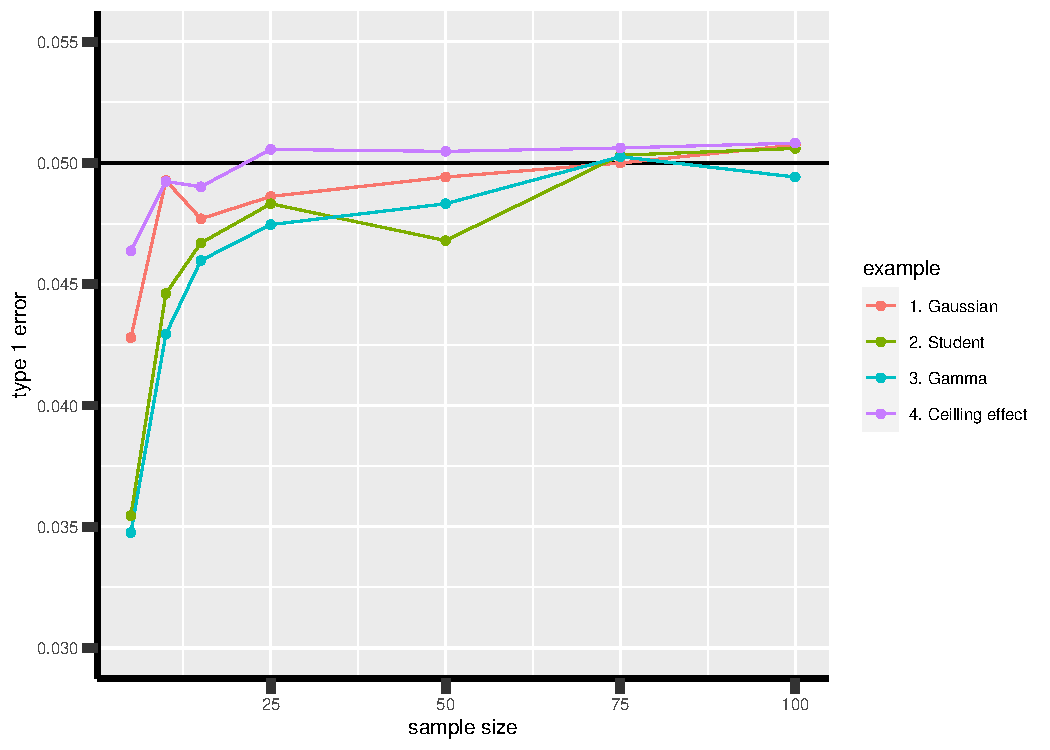
\includegraphics[width=\textwidth]{./figures/examples-coverage.pdf}
\caption{\label{fig:coverage}Coverage of the t-test.}
\end{figure}

\uline{Note:} not assuming normality complicates the understanding the group
  effect: the normal distribution is one of the few distribution that
  can be summarized by two, easily interpretable, independent,
  parameters (mean and variance).

\clearpage

\subsection{Issue 1: parameter of interest}
\label{sec:org238e88b}

By default, we generally use the mean to define our parameter of
interest. In our example the difference in mean between the two groups
meaning that we summarize the distribution of the outcome for each
group by its mean (also refered to as 'expected value') and then take the difference
between groups. This is somehow arbitrary, we could have used another
summary statistic like the standard deviation, the median (or any
other quantile), the mode, \ldots. However it is not completely arbitrary:
\begin{itemize}
\item it is \textbf{convenient} to model and compute: many estimators and softwares
have been developped for modeling the mean. Also this can be done
in a numerically stable and efficient way.
\item it is a \textbf{natural} choice if the outcome is normally distributed as
the mean and the variance fully characterize the distribution so no
need to model other summary statistics. In particular, for normal
distributions the mean is equal to the median and the mode of the
distribution.
\item it is \textbf{easy to interpret} if the outcome is normally distributed as
it is the average but also most likely value.
\end{itemize}

When the distribution is not normal, the last two arguments might not
be true. While they approximately hold if the distribution is unimodal
and symmetric, they are not valid for asymetric or bimodal
distribution. For instance, the mean of a binary variable will
correspond to a value that is never observed! If we look at
\autoref{fig:mmm}, we can see that the mean is not the most likely value
(i.e. the mode). The median is slightly closer to the mode but does
not really provide a satisfactory improvement.

\begin{figure}[!h]
\centering
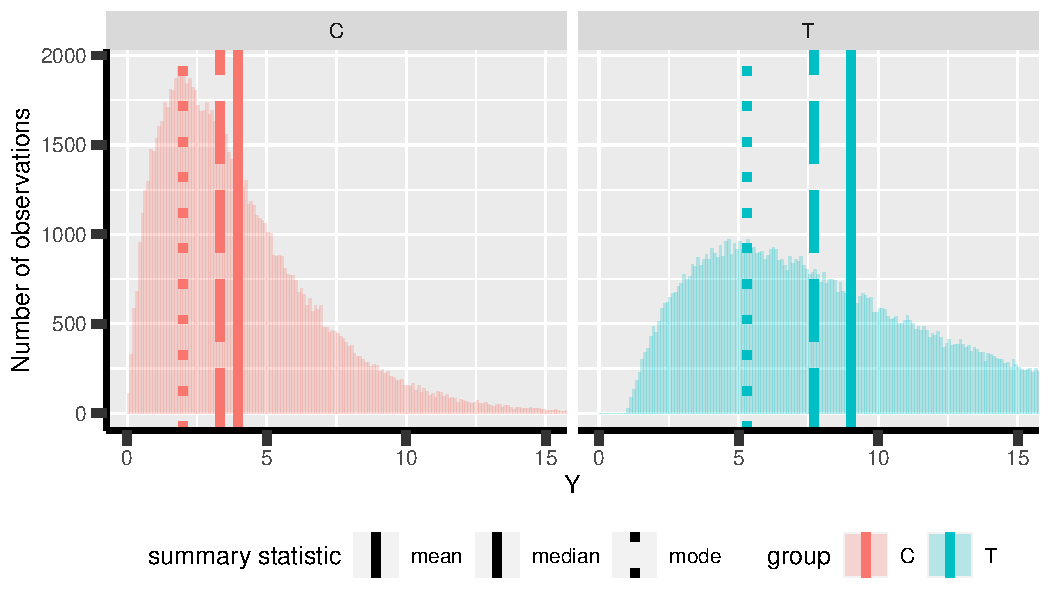
\includegraphics[width=0.85\textwidth]{./figures/meanMedianMode.pdf}
\caption{\label{fig:mmm}Mean, median, and mode two asymetric distributions.}
\end{figure}

\clearpage

 In such a case, it can be a good idea to define a new parameter of
interest. One could for instance apply a transformation that
normalizes the distribution (e.g. log-transformation, see
\autoref{fig:logmean}), estimate the mean of the transformed data (here
1.1 vs 1.8), and compare them across groups (here 0.7). In the case of
a \textbf{log-transformation}, the back-transformed difference has a nice
interpration: it is a multiplicative effect (exp(0.7)=2, i.e. the mean
in the treatment is twice larger than in the control group). So,
instead of studying an additive group effect (on the mean), \textbf{the
parameter of interest is a multiplicative group effect} (on the
mean). Technically this requires additional assumptions, such as
homoschedasticity, that are not discussed here.


\begin{figure}[!h]
\centering
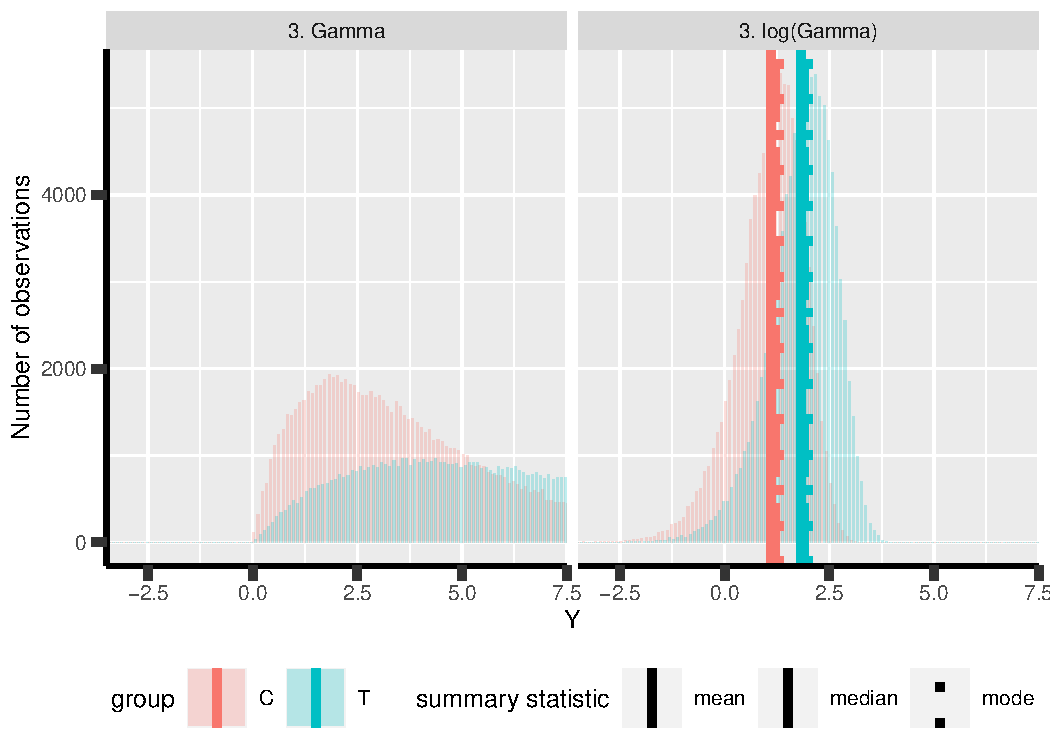
\includegraphics[width=0.85\textwidth]{./figures/logmean.pdf}
\caption{\label{fig:logmean}Mean, median, and mode on the log-transformed data}
\end{figure}

\noindent There are other possible parameter of interest, e.g.:
\begin{itemize}
\item The \textbf{Mann-Whitney parameter} \(\Prob[X\geq Y] +
  \frac{1}{2}\Prob[X=Y]\): this is the probability that a randomly
chosen individual from the active group has a larger value than a
randomly individual from the control group. 
\begin{description}
\item[{\(\rightarrow\)}] it is closely related to the
Wilcoxon-Mann-Whitney test and the AUC
\item[{\(\rightarrow\)}] not (completely) straightforward causal
interpretation \citep{fay2018causal}.
\item[{\(\rightarrow\)}] implementation: see the function \texttt{wmwTest} from
the asht package \newline \Warning in presence of
heteroschedasticity (variance that differs between groups) one
should use another tool (see the BuyseTest package)
\end{description}

\item One could dichotomize the outcome to \textbf{compare the probability of a
high outcome value} between the two groups. This can be relevant in
presence of a important ceiling effect.
\begin{description}
\item[{\(\rightarrow\)}] implementation: see the function
\texttt{uncondExact2x2} from the exact2x2 package for comparing
proportions.
\end{description}
\end{itemize}

\clearpage

\subsection{Issue 2: handling small samples}
\label{sec:org08c44f8}

In small samples, traditional methods will not provide a very accurate
type 1 error control or coverage as illustrated in
\autoref{fig:coverage}.
\begin{itemize}
\item \textbf{permutation methods} can be used to obtain exact type 1 error control
under exchangeability. Exchangeability is violated when
testing a mean difference between the groups while there is a
difference in variance. In such a case studentized permutation
should be used instead \citep{chung2016asymptotically}. \newline
\(\rightarrow\) this will produce valid p-values but no confidence
intervals
\item \textbf{bootstrap resampling methods} can be used to reduce the coverage
error error in small samples. This includes studentized
non-parametric bootstrap where the bootstrap test statistic is used
to estimate the quantiles used in the confidence intervals (instead
+/- 1.96) or bias-corrected and accelerated (BCa) bootstrap interval
(see the boot package). \newline \Warning Not all bootstrap methods
have good sample properties, e.g. the 'standard' non-parametric
bootstrap using the quantiles of the boostrap distribution of the
parameter of interest does not have very attractive small sample
properties.
\end{itemize}
There are also analytic correction for improving the small sample
properties but there typically are specific to a statistical
model/test and are not discussed here.

\subsection{Issue 3: handling outliers}
\label{sec:org7ca6472}

Most of the statistics will quantify some kind of average difference
between groups. One observation with a very large value may have large
influence on this average. If that is a concern, rank-based statistics
(e.g. median, Mann-Whitney parameter, probability of a high-value) may
be seen as more fair statistics in the sense that all observations
have the same weight on the summary statistic.
\begin{description}
\item[{\Warning}] Artificially reducing the outcome value (e.g. to be at
most the mean plus 2 standard deviation) is generally a bad idea: it
will induce a downward bias in the estimated mean and can lead to
inflated type 1 error (if the probability of a large value is group
dependent).
\end{description}

\clearpage



\section{References}
\label{sec:org42799f8}
\begingroup
\renewcommand{\section}[2]{}
\bibliographystyle{apalike}
\bibliography{bibliography}

\endgroup
\end{document}